% Generated by thesis/scripts/ch7_figures_index.py -- every Chapter 7 figure float (used, appendix, then options).
% Preamble: thesis/ch7/exp1/preview.tex (uathesis print layout). Paths as in the Overleaf upload.
\documentclass[a4paper,12pt,openany]{book}
\usepackage[a4paper,hmarginratio=1:1,vmarginratio=1:1,scale=0.75,bindingoffset=5mm]{geometry}
\usepackage{graphicx}
\usepackage{cmap}
\usepackage{amssymb}
\usepackage{amsmath}
\usepackage{setspace}
\usepackage{booktabs}
\usepackage{url}
\usepackage{adjustbox}
\usepackage{tabularx}
\usepackage{tabularray}
\usepackage{multicol}
\usepackage{subcaption}
\usepackage[inline]{enumitem}
\usepackage[table,usenames,dvipsnames]{xcolor}
\usepackage[figuresright]{rotating}  % thesis: figuresright keeps multi-page sideways floats facing one way
\usepackage{makecell}
\usepackage[unicode=true,colorlinks=true,linkcolor=black]{hyperref}
\usepackage{cleveref}
% thesis-tablestyle.tex -- one table style for the whole thesis (every chapter, generated or hand-written).
%
% Load ONCE in the preamble, after xcolor (with its `table' option) and booktabs:
%     \usepackage[table,usenames,dvipsnames]{xcolor}   % already in dissertation.tex
%     \usepackage{booktabs}                            % already in dissertation.tex
%     \input{thesis-tablestyle}
%
% What it does, in every table / table* / sidewaystable / sidewaystable* float:
%   * zebra striping of the body rows (header rows stay white), in a very light grey that prints in greyscale;
%   * slightly taller rows (\arraystretch times \thesisrowstretch, on top of any \arraystretch the table sets);
%   * booktabs rules keep their spacing; where a rule follows a shaded row, the gap above the rule is shaded
%     too, so there is no white band.
% The body starts after the first \midrule (booktabs) or the second \hline (\hline tables). Striping restarts
% after every \midrule, so a group row after a \midrule (e.g. "\multicolumn{8}{l}{\textit{PropNEAT}}") is
% white and its rows alternate below it. A table whose header ends without a \midrule says how many header
% rows it has: \thesistablestyle[1]. A table with no top rule (\toprule or \hline) is not striped.
%
% Switches (in the preamble for the whole thesis, or inside one table for that table):
%   \thesisstripestrue / \thesisstripesfalse        zebra on (default) / off
%   \thesisfiverulestrue / \thesisfiverulesfalse    thin grey rule every \thesisfiveevery body rows (default off);
%                                                   the alternative to stripes: \thesisstripesfalse\thesisfiverulestrue
%   \thesistablesautotrue / \thesistablesautofalse  apply to every table float automatically (default on); when
%                                                   off, only tables that call \thesistablestyle are styled
%   \renewcommand\thesisrowstretch{1.1}             row-height factor (1 = unchanged)
%   \renewcommand\thesisfiveevery{5}                rows between the thin rules
%   \definecolor{thesisstripe}{gray}{0.93}          stripe colour (and thesisfiverule for the thin rules)
% Per table:
%   \thesistablestyle[<n>]   apply the style (generated tables call it first; idempotent); <n> = number of
%                            header rows after \toprule when the header does not end with a \midrule
%   \thesisnostripes         opt out: this table keeps its own look (no stripes, no thin rules, no extra
%                            height). Use it for tables that colour their own cells or rows, or use \multirow
%                            (the next row's shading would cover the \multirow text).
% Nested tabulars (\makecell, a tabular inside a cell) are left alone and do not disturb the outer striping.
\makeatletter
\@ifpackageloaded{colortbl}{}{\RequirePackage{colortbl}}
\@ifpackageloaded{booktabs}{}{\RequirePackage{booktabs}}
\@ifundefined{fpeval}{\RequirePackage{xfp}}{}

\newif\ifthesisstripes   \thesisstripestrue
\newif\ifthesisfiverules \thesisfiverulesfalse
\newif\ifthesistablesauto \thesistablesautotrue
\definecolor{thesisstripe}{gray}{0.93}
\definecolor{thesisfiverule}{gray}{0.6}
\newcommand\thesisrowstretch{1.1}
\newcommand\thesisfiveevery{5}

\newif\ifthesis@active   % inside a styled float
\newif\ifthesis@engine   % stripes or thin rules are being drawn
\newif\ifthesis@data     % past the header
\newif\ifthesis@firstrule
\newif\ifthesis@lastrow  % the last item was a row (not a rule)
\newif\ifthesis@curgrey  % the current row is shaded
\newif\ifthesis@lastgrey % the row just ended was shaded
\newif\ifthesis@wantsep
\newif\ifthesis@oksep
\newcount\thesis@row     % body row number since the last \midrule (1 = first)
\newcount\thesis@five
\newcount\thesis@head    % header rows still to come (-1: wait for a \midrule)
\newcount\thesis@lvl     % group level of the outer table's \noalign (-1: unknown)
\thesis@lvl=\m@ne
\def\thesis@headrows{-1}

% ---- row colours (colortbl's per-row colour, as xcolor's \rowcolors sets it). colortbl extends each
% cell's colour by \tabcolsep on both sides; at an @{} edge that would stick out past the rules, so the
% first / last cell of a row drops that overhang when the column spec starts / ends with @{}.
\newif\ifthesis@leftflush
\newif\ifthesis@rightflush
\newcount\thesis@cellno
\newcount\thesis@ncols
% colortbl stretches a cell's colour with 1fill against the cell's own 1fill of alignment glue; a
% \makecell adds its own \hfill glue (counted in \thesis@mc), which would take part of the stretch and
% leave the right of the cell white. The colour's stretch is raised to match (\thesis@k).
\newcount\thesis@mc
\def\thesis@k{1}
\def\thesis@mcell#1#2\@nil#3{\thesis@o@mcell{#1}#2\@nil{#3}%
  \ifx\mcell@left\hfill\global\advance\thesis@mc\@ne\fi
  \ifx\mcell@right\hfill\global\advance\thesis@mc\@ne\fi}
\def\thesis@docolor{\global\let\CT@do@color\relax
  \@tempdima\wd\z@\advance\@tempdima\@tempdimb\advance\@tempdima\@tempdimc
  \kern-\@tempdimb\leaders\vrule\hskip\@tempdima\@plus\thesis@k fill
  \kern-\@tempdimc\hskip-\wd\z@\@plus-\thesis@k fill\relax}
\def\thesis@cellstep{%
  \def\thesis@k{1}%
  \ifnum\currentgrouplevel=\thesis@lvl
    \edef\thesis@k{\the\numexpr\@ne+\thesis@mc\relax}\global\thesis@mc\z@
    \global\advance\thesis@cellno\@ne
    % overlap the next cell a little, so screen renderers show no hairline gaps between cells
    \ifnum\thesis@cellno<\thesis@ncols\advance\@tempdimc.25pt\fi
    \ifnum\thesis@cellno=\@ne\ifthesis@leftflush\@tempdimb\z@\fi\fi
    \ifnum\thesis@cellno=\thesis@ncols\ifthesis@rightflush\@tempdimc\z@\fi\fi
  \fi}
\def\thesis@grey{\gdef\CT@row@color{\thesis@cellstep\CT@color{thesisstripe}}\global\thesis@curgreytrue}
\def\thesis@white{\gdef\CT@row@color{\thesis@cellstep}\global\thesis@curgreyfalse}
\ExplSyntaxOn
\cs_new_protected:Npn \thesis@edges #1
  {
    \str_set:Nn \l_tmpa_str {#1}
    \str_remove_all:Nn \l_tmpa_str { ~ }
    \str_if_eq:eeTF { \str_head:N \l_tmpa_str } { @ }
      { \global\thesis@leftflushtrue } { \global\thesis@leftflushfalse }
    \str_if_eq:eeTF { \str_range:Nnn \l_tmpa_str { -3 } { -1 } } { \tl_to_str:n { @{} } }
      { \global\thesis@rightflushtrue } { \global\thesis@rightflushfalse }
  }
\ExplSyntaxOff
\def\thesis@array[#1]#2{%
  \ifnum\thesis@lvl<\z@\thesis@edges{#2}\else\ifnum\currentgrouplevel<\thesis@lvl\thesis@edges{#2}\fi\fi
  \thesis@o@array[#1]{#2}}
\def\thesis@colour{\ifthesisstripes\ifodd\thesis@row\thesis@white\else\thesis@grey\fi\else\thesis@white\fi}
\def\thesis@startdata{\global\thesis@datatrue\global\thesis@head\m@ne\global\thesis@row\@ne
  \global\thesis@five\z@\thesis@colour}
\def\thesis@sethead{\global\thesis@lvl\currentgrouplevel\global\thesis@firstrulefalse
  \global\thesis@ncols\z@\global\thesis@cellno\z@
  \global\thesis@datafalse\global\thesis@row\z@\global\thesis@five\z@\thesis@white
  \global\thesis@head=\thesis@headrows\relax\ifnum\thesis@head=\z@\thesis@startdata\fi}

% ---- at every row end (\CT@everycr); only the outer table's rows count
\def\thesis@close{\ifnum0=`{\fi}}
\def\thesis@cr{\noalign{\ifnum0=`}\fi\thesis@crstep}
\def\thesis@crstep{\thesis@wantsepfalse
  \ifnum\currentgrouplevel=\thesis@lvl
    \ifthesis@curgrey\global\thesis@lastgreytrue\else\global\thesis@lastgreyfalse\fi
    \global\thesis@lastrowtrue
    \ifnum\thesis@cellno>\thesis@ncols\global\thesis@ncols\thesis@cellno\fi
    \global\thesis@cellno\z@\global\thesis@mc\z@
    \ifthesis@data
      \global\advance\thesis@row\@ne\thesis@colour
      \ifthesisfiverules
        \global\advance\thesis@five\@ne
        \ifnum\thesis@five<\thesisfiveevery\relax\else\global\thesis@five\z@\thesis@wantseptrue\fi
      \fi
    \else
      \thesis@white
      \ifnum\thesis@head>\z@
        \global\advance\thesis@head\m@ne
        \ifnum\thesis@head=\z@\thesis@startdata\fi
      \fi
    \fi
  \fi
  \ifthesis@wantsep\expandafter\thesis@peek\else\expandafter\thesis@close\fi}
% a thin rule after every \thesisfiveevery body rows, unless a rule or the end comes next
\def\thesis@peek{\futurenonspacelet\thesis@next\thesis@decide}
\def\thesis@nosepif#1{\ifx\thesis@next#1\thesis@oksepfalse\fi}
\def\thesis@decide{\thesis@okseptrue
  \thesis@nosepif\bottomrule\thesis@nosepif\midrule\thesis@nosepif\toprule\thesis@nosepif\cmidrule
  \thesis@nosepif\hline\thesis@nosepif\cline\thesis@nosepif\addlinespace\thesis@nosepif\specialrule
  \thesis@nosepif\end\thesis@nosepif\noalign\thesis@nosepif\crcr
  \ifthesis@oksep{\color{thesisfiverule}\hrule\@height\cmidrulewidth}\fi
  \thesis@close}

% ---- rules: #1 = 0 \cmidrule, 1 \toprule, 2 \midrule, 3 \bottomrule, 4 \hline
\def\thesis@fill{{\color{thesisstripe}\hrule\@height\aboverulesep}\vskip-\aboverulesep}
\def\thesis@rule#1{\noalign{\thesis@rulestep#1}}
\def\thesis@rulestep#1{%
  \ifnum#1=\@ne\thesis@sethead\else
  \ifnum#1=4
    \ifthesis@firstrule\thesis@sethead\else
    \ifnum\currentgrouplevel=\thesis@lvl\thesis@startdata\else\thesis@sethead\fi\fi
  \else
  \ifnum\currentgrouplevel=\thesis@lvl
    \ifthesis@lastrow\ifthesis@lastgrey\thesis@fill\fi\fi
    \ifnum#1=\tw@\thesis@startdata\fi
    \ifnum#1=\thr@@\global\thesis@datafalse\thesis@white\fi
  \fi\fi\fi
  \global\thesis@lastrowfalse}

% ---- at the start of each tabular / tabularx / tabular* (not nested ones): reset, taller rows
\def\thesis@tabbegin{%
  \ifthesis@active
    \ifnum\thesis@lvl<\z@\thesis@tabreset\else
    \ifnum\currentgrouplevel<\thesis@lvl\thesis@tabreset\fi\fi
  \fi}
\def\thesis@tabreset{\global\thesis@lvl\m@ne\global\thesis@firstruletrue\global\thesis@datafalse
  \global\thesis@row\z@\global\thesis@five\z@\global\thesis@head\m@ne\global\thesis@lastrowfalse
  \global\thesis@curgreyfalse
  \edef\arraystretch{\fpeval{\arraystretch*\thesisrowstretch}}}
\AddToHook{env/tabular/begin}{\thesis@tabbegin}
\AddToHook{env/tabular*/begin}{\thesis@tabbegin}
\AddToHook{env/tabularx/begin}{\thesis@tabbegin}

% ---- the style itself
\newcommand\thesistablestyle[1][-1]{%
  \def\thesis@headrows{#1}%
  \ifthesis@active\else
    \thesis@activetrue\global\thesis@lvl\m@ne
    \thesis@enginefalse
    \ifthesisstripes\thesis@enginetrue\fi
    \ifthesisfiverules\thesis@enginetrue\fi
    \ifthesis@engine
      \CT@everycr{\the\everycr\thesis@cr}%
      \let\thesis@o@toprule\toprule\def\toprule{\thesis@rule1\thesis@o@toprule}%
      \let\thesis@o@midrule\midrule\def\midrule{\thesis@rule2\thesis@o@midrule}%
      \let\thesis@o@bottomrule\bottomrule\def\bottomrule{\thesis@rule3\thesis@o@bottomrule}%
      \let\thesis@o@cmidrule\cmidrule\def\cmidrule{\thesis@rule0\thesis@o@cmidrule}%
      \let\thesis@o@hline\hline\def\hline{\thesis@rule4\thesis@o@hline}%
      \ifdefined\@@array\let\thesis@o@array\@@array\let\@@array\thesis@array\fi
      \ifdefined\mcell@@@tabular\let\thesis@o@mcell\mcell@@@tabular\let\mcell@@@tabular\thesis@mcell\fi
      \let\thesis@o@docolor\CT@@do@color\let\CT@@do@color\thesis@docolor
    \fi
  \fi}
\newcommand\thesisnostripes{%
  \ifthesis@active
    \thesis@activefalse
    \ifthesis@engine
      \CT@everycr{\noalign{\global\let\CT@row@color\relax}\the\everycr}%
      \let\toprule\thesis@o@toprule\let\midrule\thesis@o@midrule\let\bottomrule\thesis@o@bottomrule
      \let\cmidrule\thesis@o@cmidrule\let\hline\thesis@o@hline
      \ifdefined\thesis@o@array\let\@@array\thesis@o@array\fi
      \ifdefined\thesis@o@mcell\let\mcell@@@tabular\thesis@o@mcell\fi
      \let\CT@@do@color\thesis@o@docolor
      \thesis@enginefalse
    \fi
  \fi}
\def\thesis@auto{\ifthesistablesauto\thesistablestyle\fi}
\AddToHook{env/table/begin}{\thesis@auto}
\AddToHook{env/table*/begin}{\thesis@auto}
\AddToHook{env/sidewaystable/begin}{\thesis@auto}
\AddToHook{env/sidewaystable*/begin}{\thesis@auto}
\makeatother
  % thesis table style (loaded once in the thesis preamble)
\newcolumntype{Y}{>{\centering\arraybackslash}X}
\renewcommand\floatpagefraction{.9}
\renewcommand\topfraction{.9}
\renewcommand\bottomfraction{.9}
\renewcommand\textfraction{.1}
\setcounter{totalnumber}{50}
\setcounter{topnumber}{50}
\setcounter{bottomnumber}{50}
\begin{document}
\chapter*{Chapter 7 figures: used}
% Generated by thesis/ch7/exp1/make_figures.py -- do not edit by hand.
\begin{figure}[tbp]
  \centering
  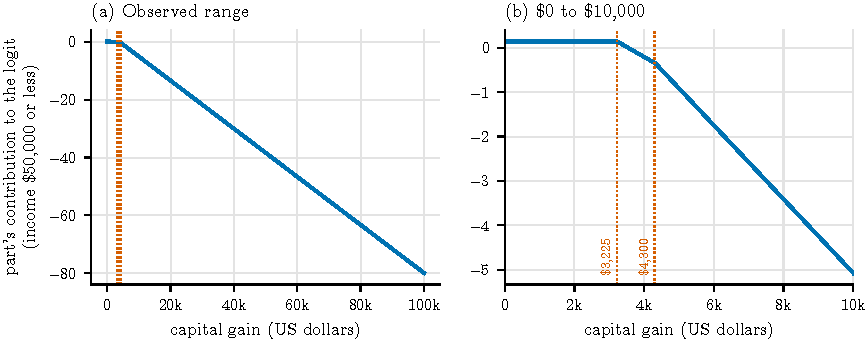
\includegraphics[width=\textwidth,height=0.8\textheight,keepaspectratio]{figures/ch7/adult-capgain-response.pdf}
  \caption{Adult, original network: response of the part \emph{Capital gains} to capital gain. Blue: the part's contribution to the output logit (log-odds of an income of \$50,000 or less), its country-of-birth inputs at 0; dotted red: the knots of the piecewise-linear response.}
  \label{fig:ch7-adult-capgain-response}
\end{figure}

% Generated by thesis/ch7/exp1/bench_figures.py -- do not edit by hand.
\begin{figure}[tbp]
  \centering
  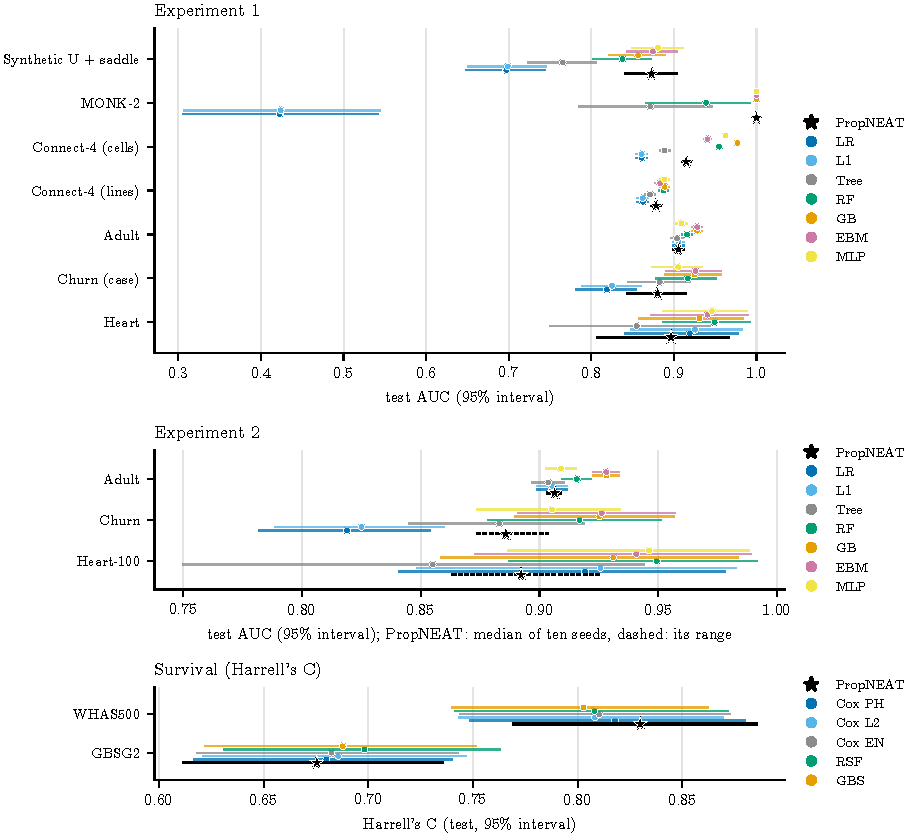
\includegraphics[width=\textwidth,height=0.8\textheight,keepaspectratio]{figures/ch7/bench-dots.pdf}
  \caption{Test AUC of PropNEAT and of each comparator, every dataset. Star: PropNEAT (Experiment 2: median of the ten seeds, dashed: their range); dots: comparators; lines: 95\% intervals; survival datasets: Harrell's C. LR: logistic regression ($L_2$); L1: $L_1$ logistic regression; RF: random forest; GB: gradient boosting; EBM: explainable boosting machine; MLP: multilayer perceptron; Cox L2 / Cox EN: Cox model with a ridge / elastic-net penalty; RSF: random survival forest; GBS: gradient-boosted survival model.}
  \label{fig:ch7-bench-dots}
\end{figure}

\clearpage
% Generated by thesis/ch7/exp1/c4_case_figures.py -- do not edit by hand.
\begin{figure}[tbp]
  \centering
  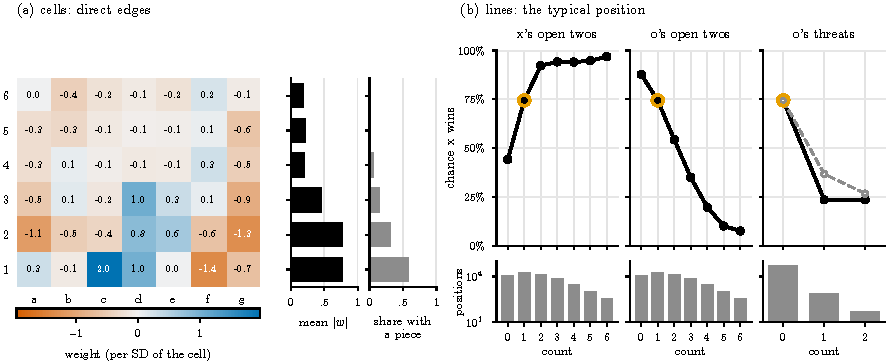
\includegraphics[width=\textwidth,height=0.8\textheight,keepaspectratio]{figures/ch7/c4-case-contrast.pdf}
  \caption{Connect-4: the cells network's direct edges and the lines network's response. (a) Cells network: the weight of each cell's direct edge to the output (blue raises the chance that x wins, red lowers it; row 1 is the bottom of the board); bars: per row, the mean absolute weight (black) and the share of training positions with a piece on a cell of the row (grey). (b) Lines network: the predicted chance that x wins as one line feature changes, all others at the typical position (orange circle); o's threats: solid, every threat on an even row; dashed, the threat count alone, its row parity left at zero. Grey bars: training positions at each count (log scale).}
  \label{fig:ch7-c4-case-contrast}
\end{figure}

% Generated by thesis/ch7/exp1/churn_case_figures.py -- do not edit by hand.
\begin{figure}[tbp]
  \centering
  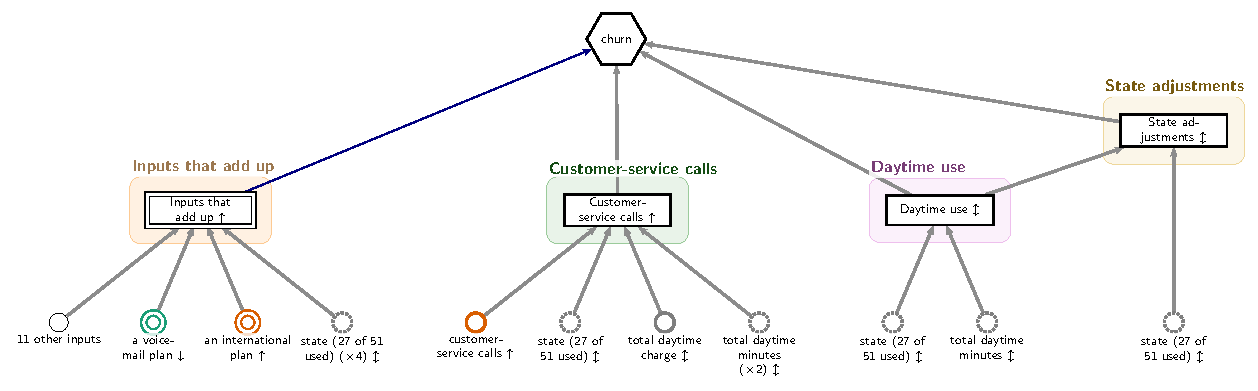
\includegraphics[width=\textwidth,height=0.8\textheight,keepaspectratio]{figures/ch7/churn-case-net-concept.pdf}
  \caption{Churn case network (seed 10) at the level of its parts. Each top-level part of the explanation is one box, with the inputs it reads below it and the churn score at the top. Arrows on inputs and boxes: the direction of the effect on the final prediction (up raises it, down lowers it, double arrow depends). Edges: blue, a positive weight (raises the score); red, a negative weight; thicker, a larger weight; grey, no single weight (the inputs a collapsed part reads, and a part's sum). Double outline: acts at a fixed rate everywhere (dashed double: on the observed data). A grouped input (state) stands for its used levels; \emph{11 other inputs}: the rest of the inputs of \emph{Inputs that add up}.}
  \label{fig:ch7-churn-case-net-concept}
\end{figure}

\clearpage
% Generated by thesis/ch7/exp1/churn_case_figures.py -- do not edit by hand.
\begin{figure}[tbp]
  \centering
  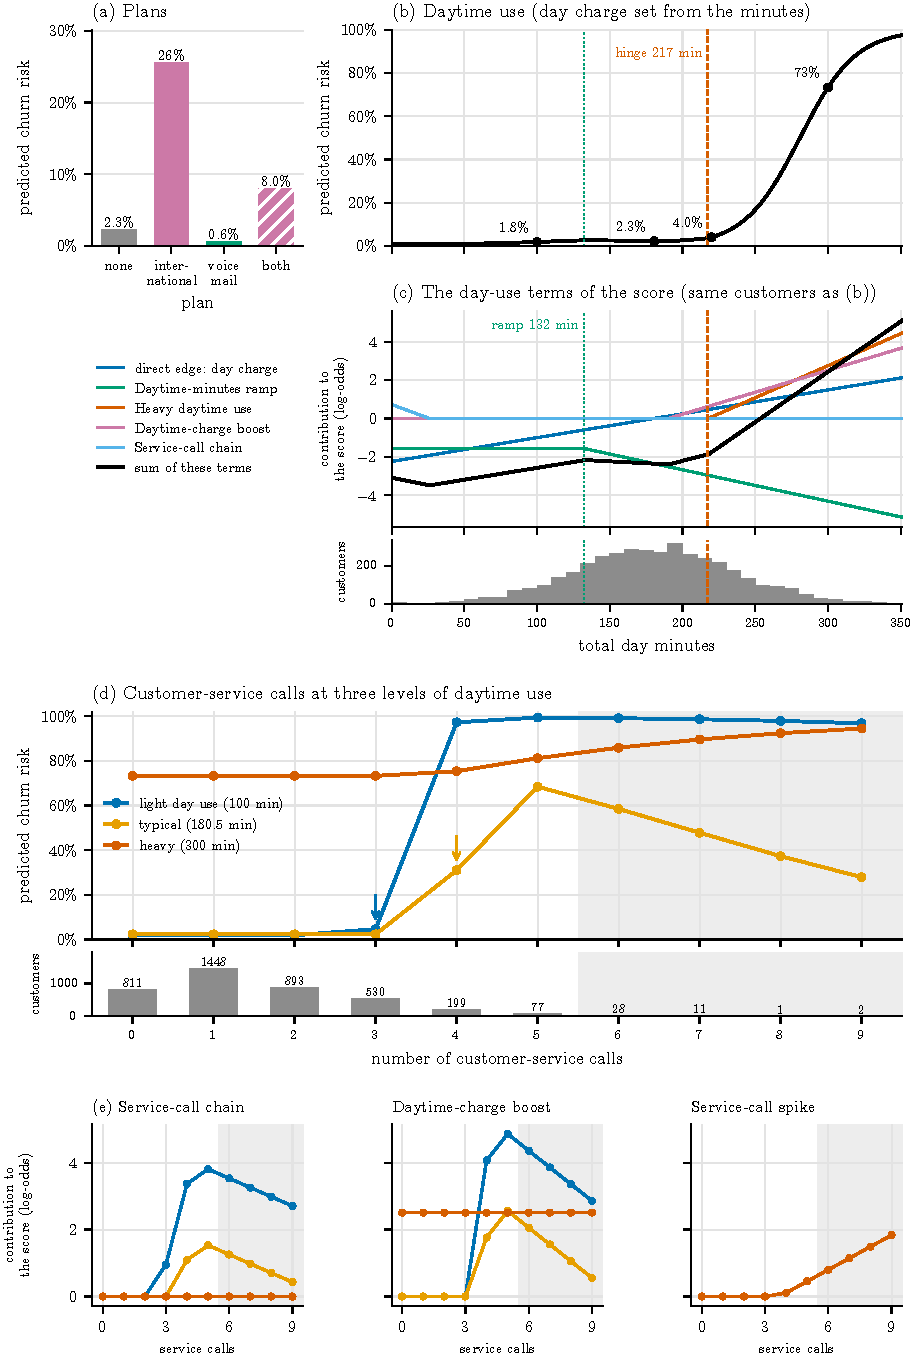
\includegraphics[width=\textwidth,height=0.85\textheight,keepaspectratio]{figures/ch7/churn-case-probes.pdf}
  \caption{Churn case network (seed 10): predicted churn risk of the typical customer as inputs change. (a) The plans (hatched: both). (b) Black: risk against daytime use, the day charge set from the minutes; dots: 100, 180.5, 220, 300 minutes; dashed red: where the part \emph{Heavy daytime use} switches on; grey bars: training customers per 10 minutes. (c) Risk against customer-service calls at three levels of daytime use (colours); arrow: the call count at which the part \emph{Service-call chain} switches on; grey bars: training customers per call count; shaded: fewer than 50 training customers. (d) The three service-call parts' contributions to the score (log-odds) over the same calls, colours as in (c); a line not visible lies under another.}
  \label{fig:ch7-churn-case-probes}
\end{figure}

% Generated by thesis/ch7/exp2/make_assets.py -- do not edit by hand.
\begin{figure}[tbp]
  \centering
  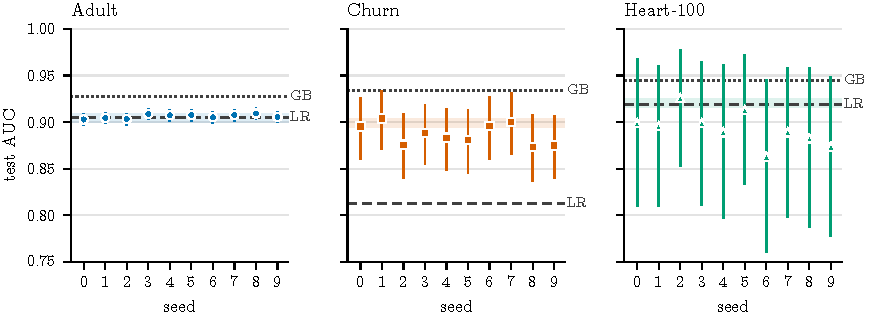
\includegraphics[width=\textwidth,height=0.8\textheight,keepaspectratio]{figures/ch7/used/exp2-auc}
  \caption{Test AUC of each seed's network, with its 95\% interval. Shaded: within 0.01 of the best seed. Dashed: logistic regression (LR); dotted: gradient boosting (GB).}
  \label{fig:exp2-auc}
\end{figure}

\clearpage
% Generated by thesis/ch7/exp2/make_assets.py -- do not edit by hand.
\begin{figure}[tbp]
  \centering
  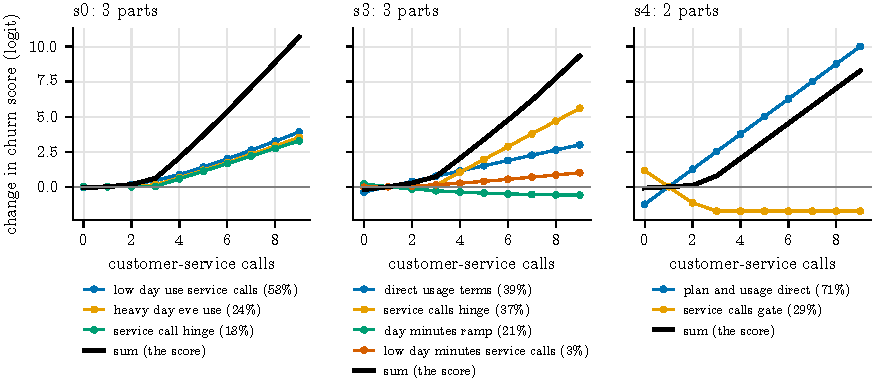
\includegraphics[width=\textwidth,height=0.8\textheight,keepaspectratio]{figures/ch7/used/exp2-churn-calls-parts}
  \caption{Churn: one signal, three realisations. The score's response to customer-service calls (relative to 1 call), split into the explanation parts that carry it; black: their sum, the score's response. Legend: each part's share of the response's variance.}
  \label{fig:exp2-churn-calls-parts}
\end{figure}

% Generated by thesis/ch7/exp2/make_assets.py -- do not edit by hand.
\begin{figure}[tbp]
  \centering
  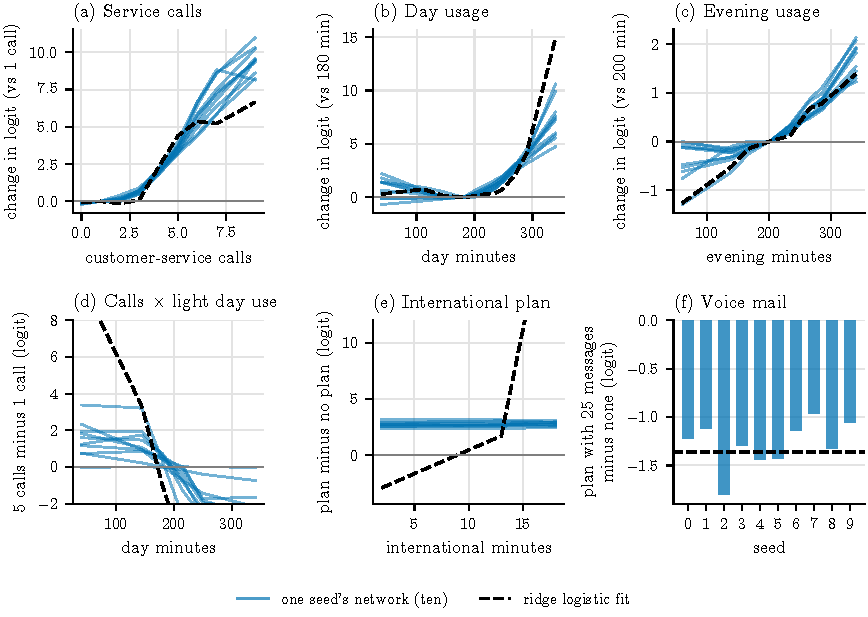
\includegraphics[width=\textwidth,height=0.8\textheight,keepaspectratio]{figures/ch7/exp2-churn-shapes.pdf}
  \caption{Churn: each signal's shape in the ten networks, as a change in the churn score (logit). Blue: one seed's network (one line or bar per seed); dashed: ridge logistic fit.}
  \label{fig:exp2-churn-shapes}
\end{figure}

\clearpage
% Generated by thesis/ch7/exp2/make_assets.py -- do not edit by hand.
\begin{figure}[tbp]
  \centering
  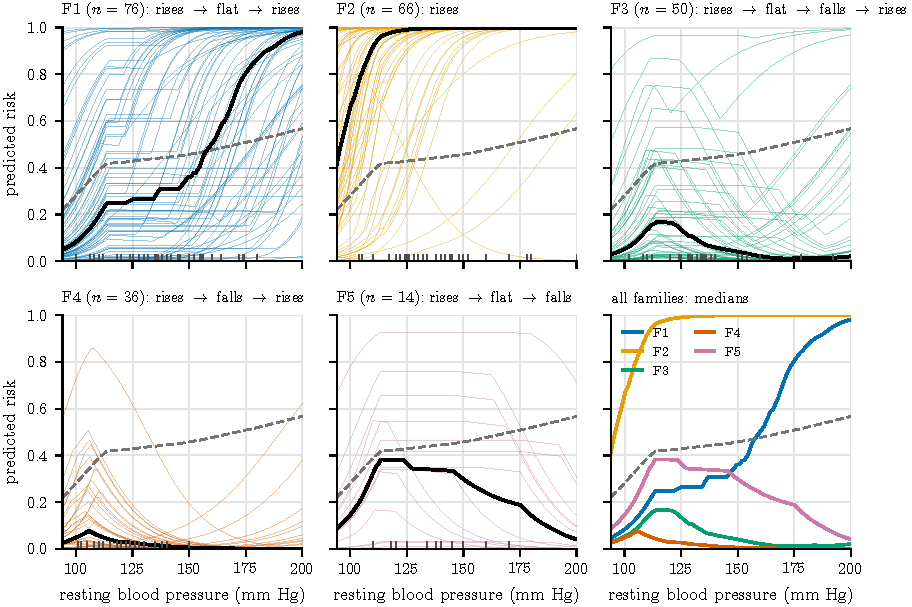
\includegraphics[width=\textwidth,height=0.8\textheight,keepaspectratio]{figures/ch7/used/exp2-s8-ice}
  \caption{Heart-100 seed 8: individual conditional expectation (ICE) curves of predicted risk against resting blood pressure, one panel per shape family. Thin coloured: one training patient; black: the family's median curve; grey dashed: mean of all curves; ticks on the axis: the family's own blood pressures. Last panel: the family medians together.}
  \label{fig:exp2-s8-ice}
\end{figure}

% Generated by thesis/ch7/exp2/worked.py -- do not edit by hand.
\begin{figure}[tbp]
  \centering
  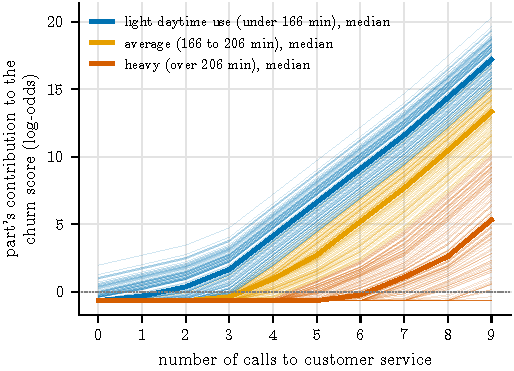
\includegraphics[width=0.7\textwidth,height=0.8\textheight,keepaspectratio]{figures/ch7/exp2-worked-ice.pdf}
  \caption{Churn seed 5, the part \emph{Service calls and daytime charge}: individual conditional expectation (ICE) curves of the part's contribution to the churn score as the number of customer-service calls varies, coloured by the customer's daytime minutes (thirds), with the median curve of each third. 0: the part adds nothing beyond its average.}
  \label{fig:exp2-worked-ice}
\end{figure}

\clearpage
% Generated by thesis/ch7/exp2/worked.py -- do not edit by hand.
\begin{figure}[tbp]
  \centering
  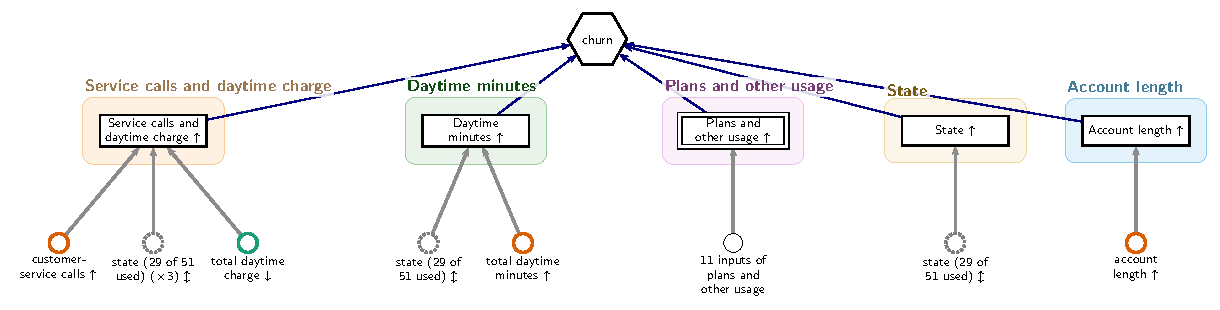
\includegraphics[width=\textwidth,height=0.8\textheight,keepaspectratio]{figures/ch7/used/exp2-worked-net-concept}
  \caption{Churn seed 5 at the level of concepts: each top-level part of the explanation collapsed into one box, the inputs each reads, and the churn score at the top. Arrows on inputs and boxes: the direction of the effect on the final prediction (up raises it, down lowers it, double arrow depends). Edges: blue, a positive weight (raises the score); red, a negative weight; thicker, a larger weight; grey, the inputs a collapsed part reads (no single weight). A grouped input (state) stands for its used levels.}
  \label{fig:exp2-worked-net-concept}
\end{figure}

% Generated by thesis/ch7/exp2/worked.py -- do not edit by hand.
\begin{figure}[tbp]
  \centering
  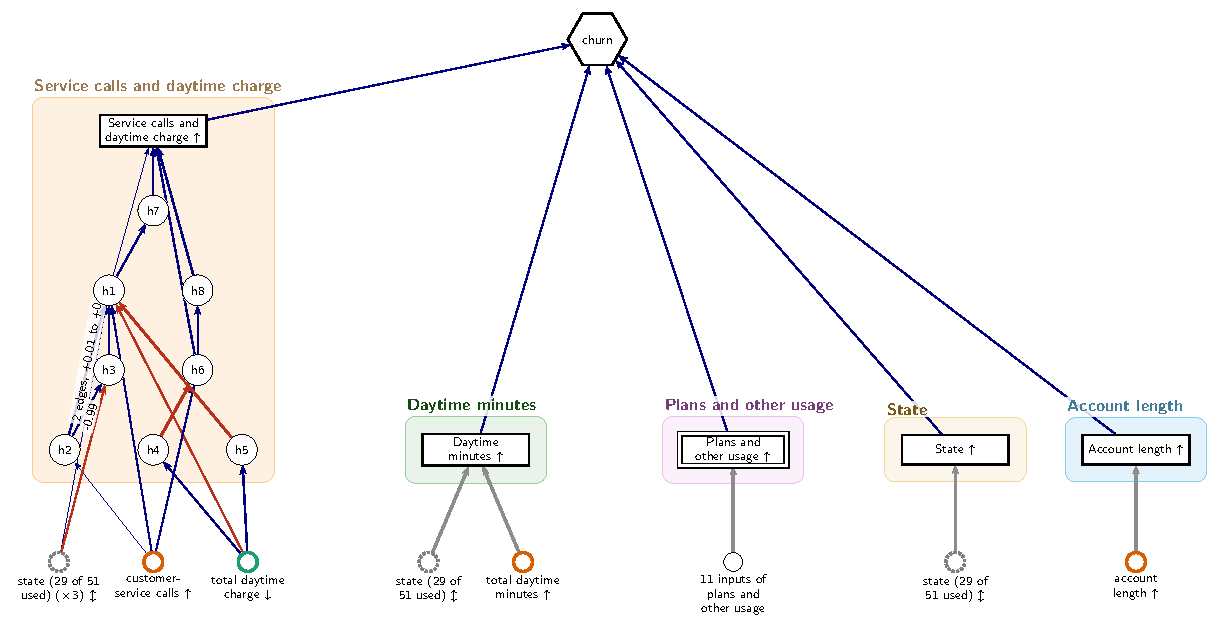
\includegraphics[width=\textwidth,height=0.8\textheight,keepaspectratio]{figures/ch7/used/exp2-worked-net-exploded}
  \caption{Churn seed 5 with the part \emph{Service calls and daytime charge} expanded and the other parts collapsed. Edges: blue, a positive weight (raises the score); red, a negative weight; thicker, a larger weight; grey, the inputs a collapsed part reads (no single weight).}
  \label{fig:exp2-worked-net-exploded}
\end{figure}

\clearpage
% Generated by thesis/ch7/exp2/worked.py -- do not edit by hand.
\begin{figure}[tbp]
  \centering
  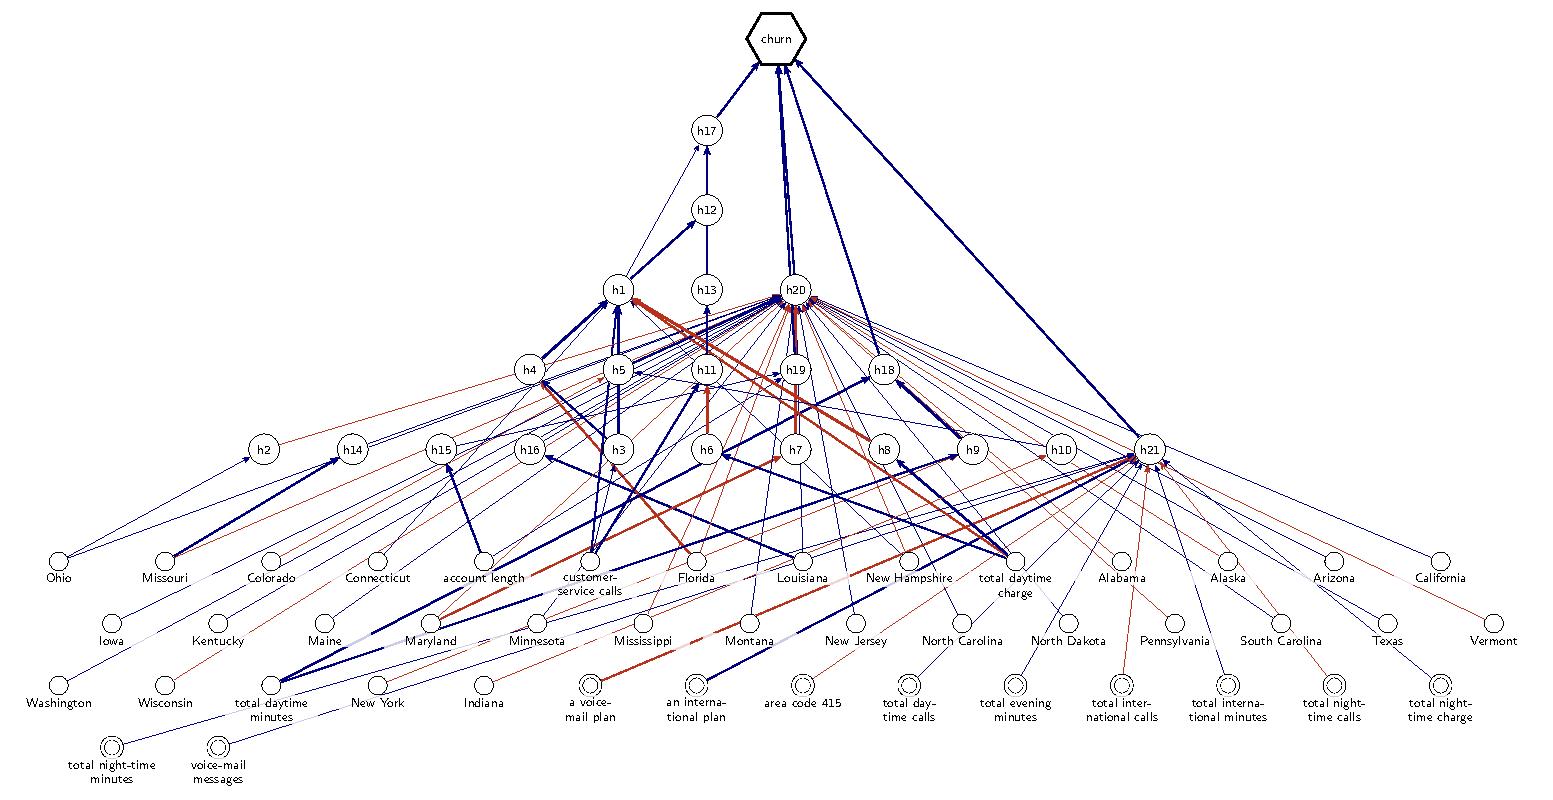
\includegraphics[width=\textwidth,height=0.8\textheight,keepaspectratio]{figures/ch7/exp2-worked-net-unexplained.pdf}
  \caption{Churn seed 5 as trained, before any explanation: input columns (bottom), hidden units (circles) and the output (hexagon). Edges: blue, a positive weight (raises the score); red, a negative weight; thicker, a larger weight. Double outline: an input that acts at a fixed rate.}
  \label{fig:exp2-worked-net-unexplained}
\end{figure}

% Generated by thesis/ch7/exp2/worked.py -- do not edit by hand.
\begin{figure}[tbp]
  \centering
  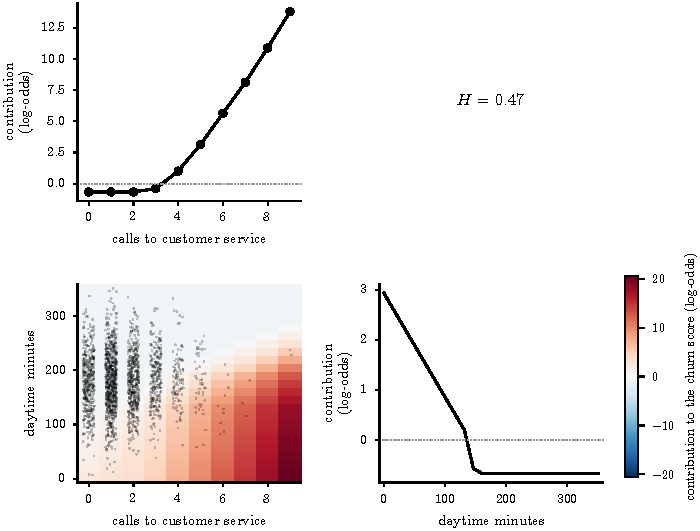
\includegraphics[width=0.85\textwidth,height=0.8\textheight,keepaspectratio]{figures/ch7/used/exp2-worked-pairs}
  \caption{Churn seed 5, the part \emph{Service calls and daytime charge}: a pairs plot of the part's contribution to the churn score (log-odds) over its two main inputs. Diagonal: one input varies; lower left: both together (colour: blue lowers and red raises the score; dots: training customers, calls jittered); upper right: the interaction strength $H$. The daytime charge is drawn in minutes.}
  \label{fig:exp2-worked-pairs}
\end{figure}

\clearpage
% Generated by thesis/ch7/exp2/exp2_figures.py -- do not edit by hand.
\begin{figure}[tbp]
  \centering
  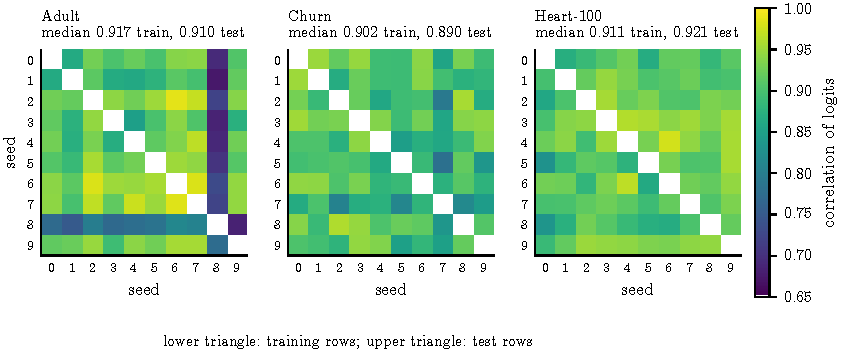
\includegraphics[width=\textwidth,height=0.8\textheight,keepaspectratio]{figures/ch7/seed-agreement.pdf}
  \caption{Pairwise correlation of the ten networks' logits. Lower triangle: training rows; upper triangle: test rows; colour: correlation.}
  \label{fig:ch7-seed-agreement}
\end{figure}

% Generated by thesis/ch7/exp2/exp2_figures.py -- do not edit by hand.
\begin{figure}[tbp]
  \centering
  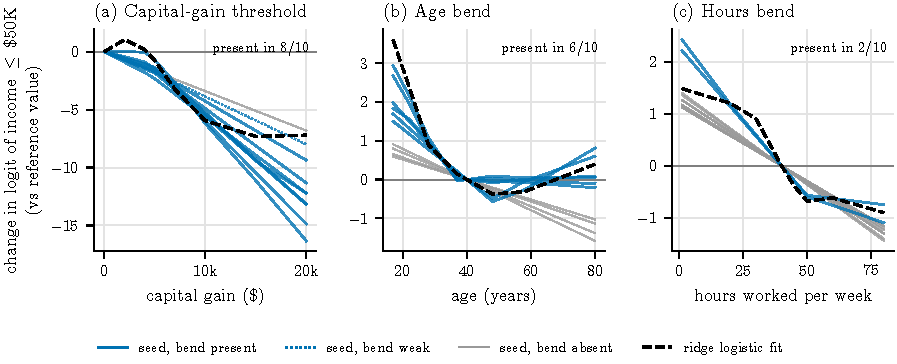
\includegraphics[width=\textwidth,height=0.8\textheight,keepaspectratio]{figures/ch7/used/sig-shapes-adult}
  \caption{Adult: shapes of the non-linear signals, one line per seed. Solid blue: a seed with the bend present; dotted blue: weak; grey: absent; dashed black: ridge logistic fit.}
  \label{fig:ch7-sig-shapes-adult}
\end{figure}

\clearpage
% Generated by thesis/ch7/exp1/make_figures.py -- do not edit by hand.
\begin{figure}[p]
  \centering
  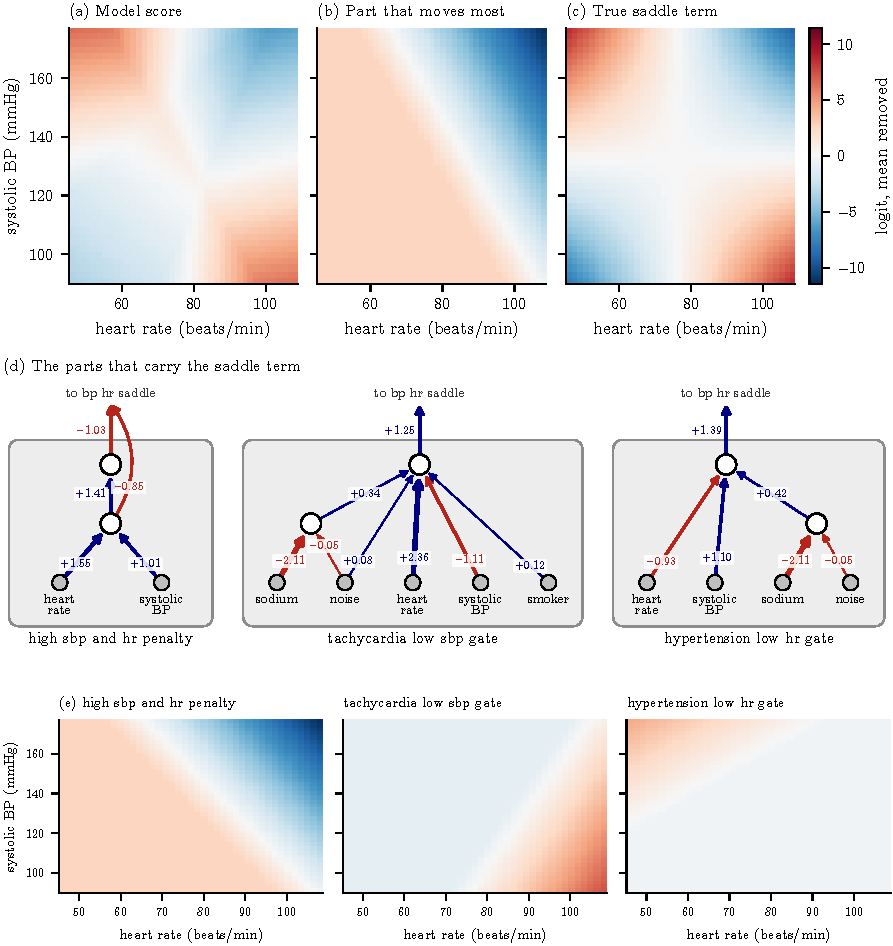
\includegraphics[width=\textwidth,height=0.77\textheight,keepaspectratio]{figures/ch7/synthetic-shape-c-saddle.pdf}
  \caption{Synthetic U + saddle network (seed 4): the heart-rate $\times$ systolic-pressure saddle term. (a, b, f) The logit with its mean over the grid removed, one scale (red above, blue below); every other input at the typical case; true term $-1.5\,z_h z_p$. (c, d) (a) minus (b): (c) the size of the gap (pale: they agree); (d) its sign (brown: model above the truth; teal: below). Dots: the training rows. (e) The parts that carry the term: grey box, one part (name below); grey circles, its inputs; white circles, ReLU units; square $+$, the part's sum. Edges: blue positive, red negative, width and label the weight; arrows leaving a box, its connections to the rest of the network. (f) Each part of (e), left to right: its contribution to the logit.}
  \label{fig:ch7-synthetic-shape-c-saddle}
\end{figure}

% Generated by thesis/ch7/exp1/make_figures.py -- do not edit by hand.
\begin{figure}[tbp]
  \centering
  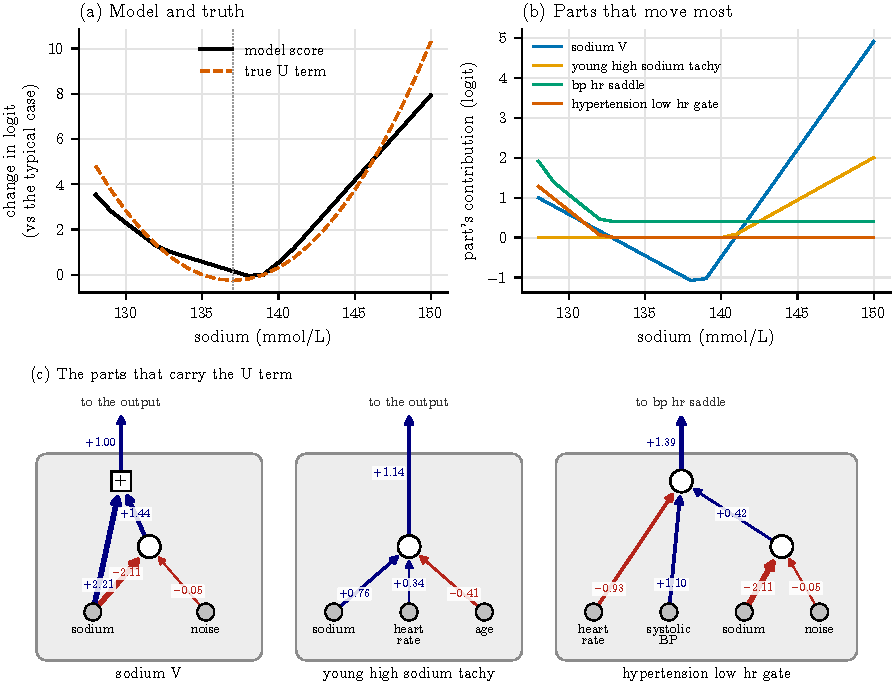
\includegraphics[width=\textwidth,height=0.8\textheight,keepaspectratio]{figures/ch7/synthetic-shape-c-sodium.pdf}
  \caption{Synthetic U + saddle network (seed 4): the U-shaped sodium term. (a) Black: the model's score as sodium varies, every other input at the typical case, relative to the typical sodium; dashed: the true U term $((z_n - (-0.5))^2 - 1)$, lowest at 137 mmol/L; dotted: 137 mmol/L. (b) The explanation parts whose contribution moves most with sodium. (c) The network's parts that carry the U term: grey box: one part of the explanation (its name below); small grey circles: the inputs it reads; white circles: hidden units (ReLU); square $+$: the part's sum (no activation). Edges: blue, a positive weight; red, a negative weight; thicker, a larger weight; the number on an edge is its weight. Arrows leaving a box: the part's connections to the rest of the network, labelled with what they feed.}
  \label{fig:ch7-synthetic-shape-c-sodium}
\end{figure}

\clearpage
% Generated by thesis/ch7/exp2/exp2_figures.py -- do not edit by hand.
\begin{figure}[tbp]
  \centering
  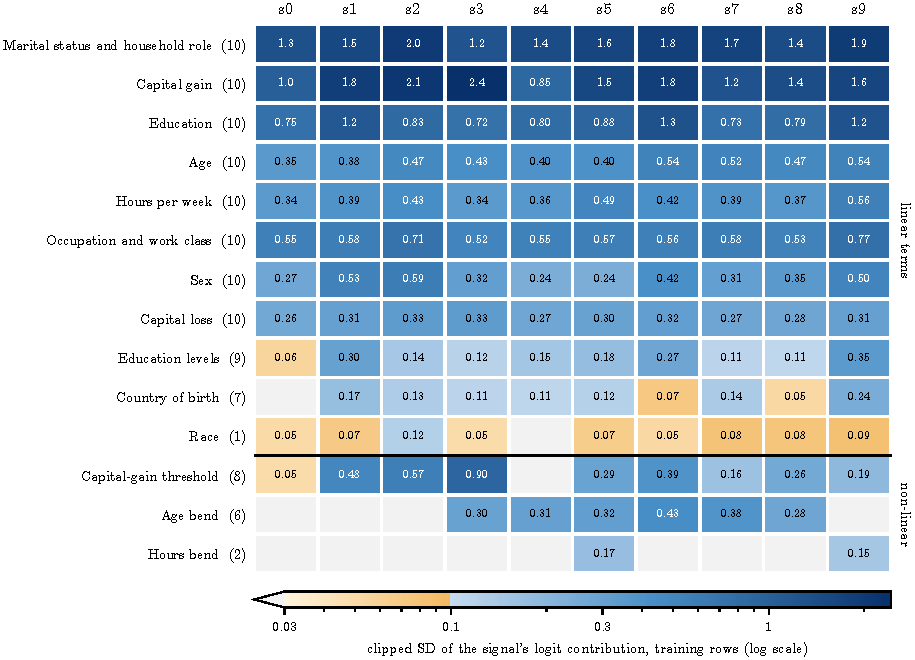
\includegraphics[width=\textwidth,height=0.8\textheight,keepaspectratio]{figures/ch7/tickmap-adult.pdf}
  \caption{Adult: size of each signal in each seed's network. Shade: clipped SD of the signal's logit contribution (training rows, log scale); blue: present ($\geq$ 0.10); orange: weak (0.03--0.10); grey: below 0.03. (n): seeds where present; red box: opposite direction to most seeds; $\cdot$: input not read. Below the line: non-linear signals.}
  \label{fig:ch7-tickmap-adult}
\end{figure}

% Generated by thesis/ch7/exp2/exp2_figures.py -- do not edit by hand.
\begin{figure}[tbp]
  \centering
  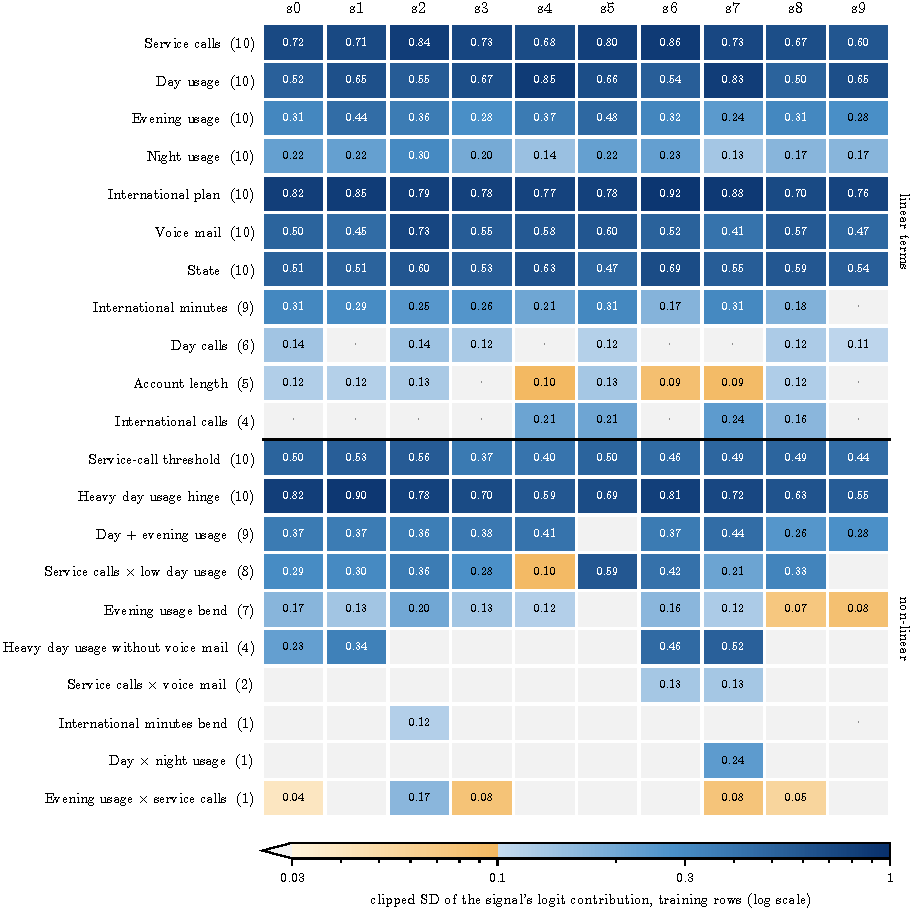
\includegraphics[width=\textwidth,height=0.8\textheight,keepaspectratio]{figures/ch7/tickmap-churn.pdf}
  \caption{Churn: size of each signal in each seed's network. Shade: clipped SD of the signal's logit contribution (training rows, log scale); blue: present ($\geq$ 0.10); orange: weak (0.03--0.10); grey: below 0.03. (n): seeds where present; red box: opposite direction to most seeds; $\cdot$: input not read. Below the line: non-linear signals.}
  \label{fig:ch7-tickmap-churn}
\end{figure}

\clearpage
% Generated by thesis/ch7/exp2/exp2_figures.py -- do not edit by hand.
\begin{figure}[tbp]
  \centering
  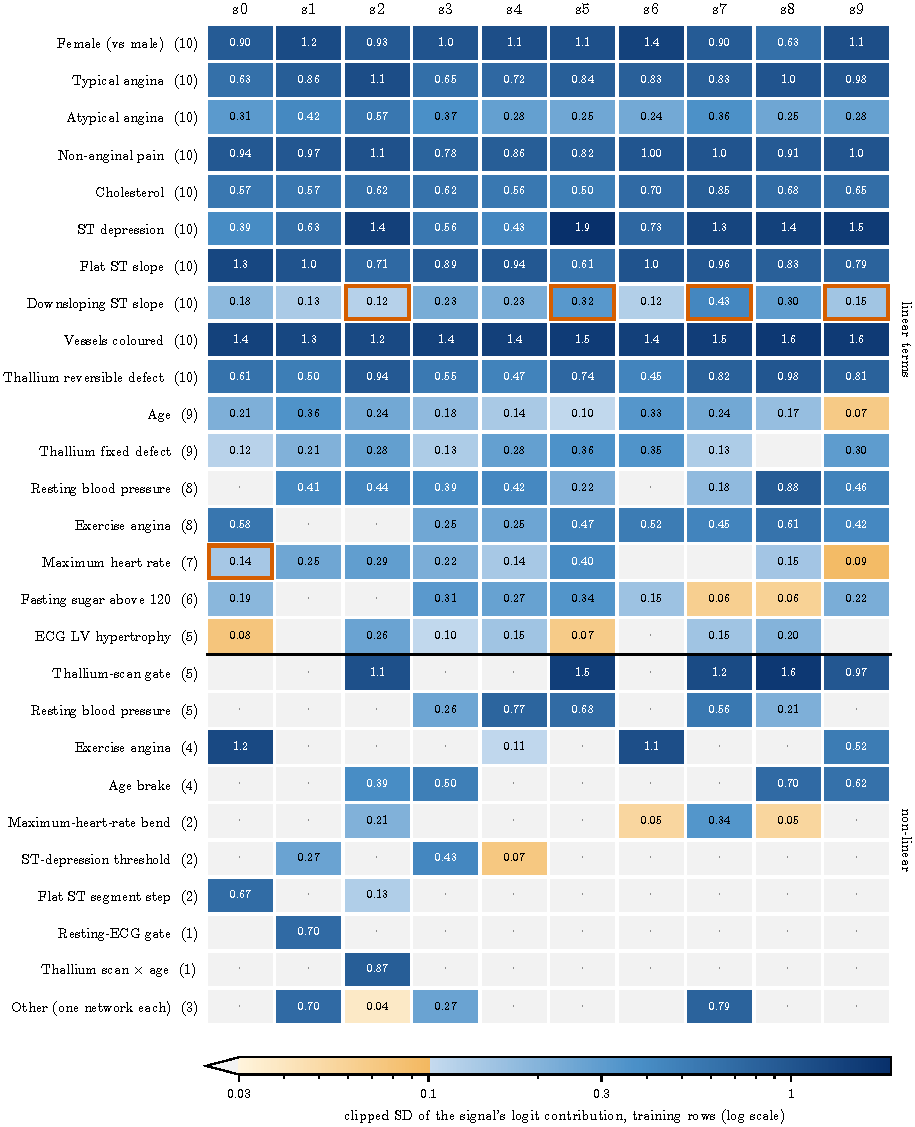
\includegraphics[width=\textwidth,height=0.8\textheight,keepaspectratio]{figures/ch7/tickmap-heart100.pdf}
  \caption{Heart-100: size of each signal in each seed's network. Shade: clipped SD of the signal's logit contribution (training rows, log scale); blue: present ($\geq$ 0.10); orange: weak (0.03--0.10); grey: below 0.03. (n): seeds where present; red box: opposite direction to most seeds; $\cdot$: input not read; for a family row, no such unit. Below the line: non-linear signals.}
  \label{fig:ch7-tickmap-heart100}
\end{figure}

% Generated by thesis/ch7/exp2/exp2_figures.py -- do not edit by hand.
\begin{figure}[tbp]
  \centering
  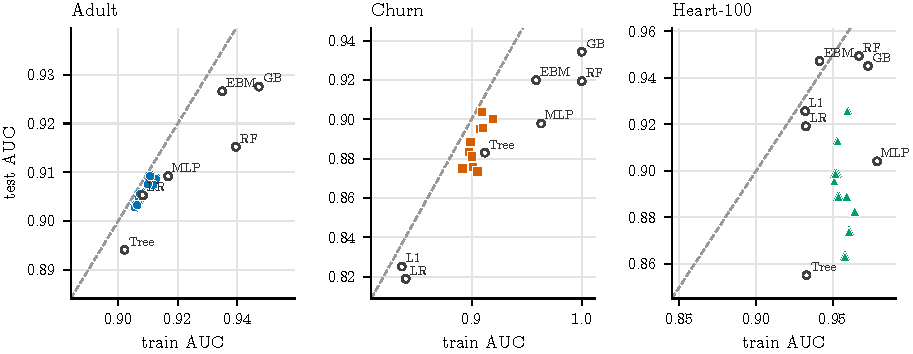
\includegraphics[width=\textwidth,height=0.8\textheight,keepaspectratio]{figures/ch7/train-vs-test-auc.pdf}
  \caption{Training against test AUC: the ten seeds and the comparators. Filled marks: the ten seeds; open circles: comparators (LR: logistic regression, $L_2$; L1: $L_1$ logistic regression; RF: random forest; GB: gradient boosting; EBM: explainable boosting machine; MLP: multilayer perceptron); dashed: training AUC = test AUC.}
  \label{fig:ch7-train-vs-test-auc}
\end{figure}

\clearpage
% Generated by thesis/ch7/exp1/make_figures.py -- do not edit by hand.
\begin{figure}[p]
  \centering
  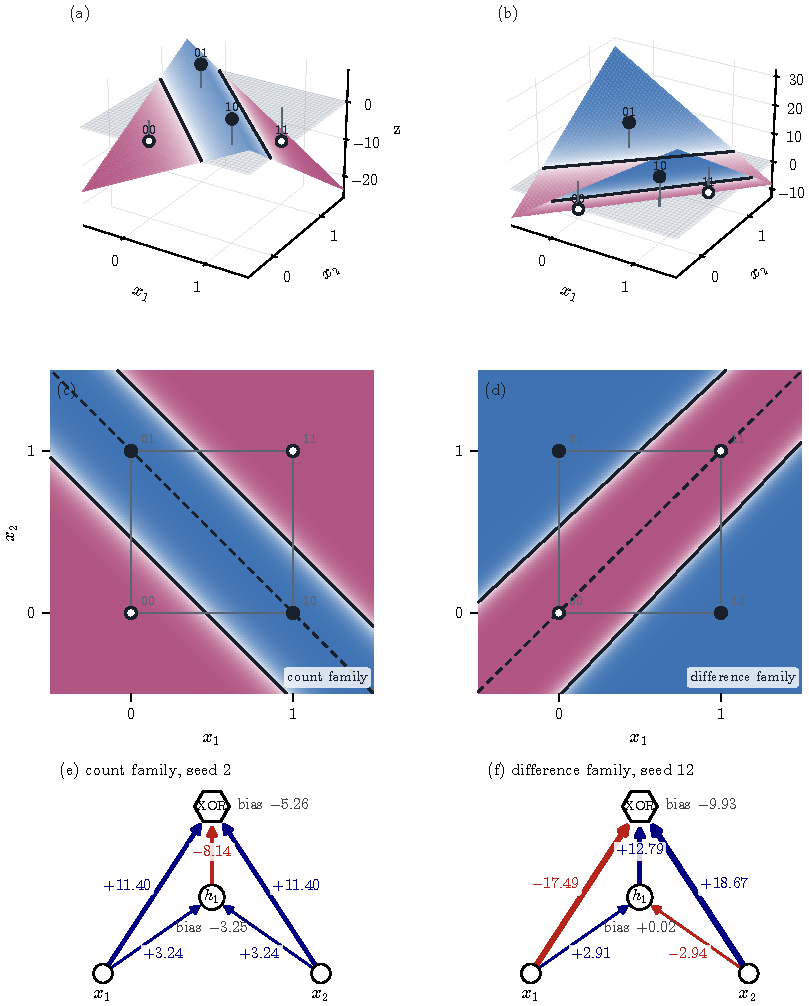
\includegraphics[width=\textwidth,height=0.77\textheight,keepaspectratio]{figures/ch7/xor-ridge-valley.pdf}
  \caption{XOR: one network of each family, the count family (a, c, e; seed 2) and the difference family (b, d, f; seed 12). (a, b) The score surface $z(x_1, x_2)$ over the plane $z = 0$ (grey); (c, d) the same scores from above. Shading: blue where the score is positive, magenta where it is negative, pale near 0; solid line: where it is 0. Filled points: the two inputs with XOR output 1; dashed line: the hidden unit's fold. (e, f) The networks of (a--d): circles $x_1$, $x_2$: the inputs; circle $h_1$: the hidden unit (ReLU); hexagon: the output unit, the logistic function of the score $z$. Edges: blue, a positive weight; red, a negative weight; thicker, a larger weight. The number on an edge is its weight; beside a unit, its bias.}
  \label{fig:ch7-xor-ridge-valley}
\end{figure}

\clearpage
\chapter*{Chapter 7 figures: appendix}
% Generated by thesis/ch7/exp1/make_figures.py -- do not edit by hand.
\begin{figure}[tbp]
  \centering
  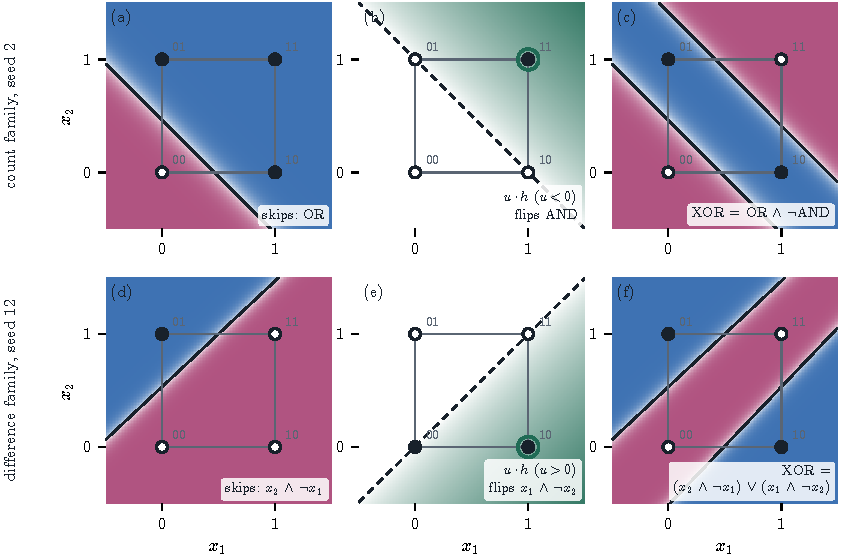
\includegraphics[width=\textwidth,height=0.8\textheight,keepaspectratio]{figures/ch7/xor-gates.pdf}
  \caption{XOR: the gates of each family, count family (a--c) and difference family (d--f). Left: the skip connections alone; middle: the hidden unit's contribution $u\cdot h$ (green: active, darker for larger $|u h|$; dashed: its fold; ringed points: the inputs whose sign it flips); right: the composed score. Shading: blue where the score is positive, magenta where it is negative, pale near 0; solid line: where it is 0. Filled points: inputs where the panel's quantity is positive (middle: where the hidden unit is active).}
  \label{fig:ch7-xor-gates}
\end{figure}

\clearpage
\chapter*{Chapter 7 figures: options}
% Generated by thesis/ch7/exp1/make_figures.py -- do not edit by hand.
\begin{figure}[tbp]
  \centering
  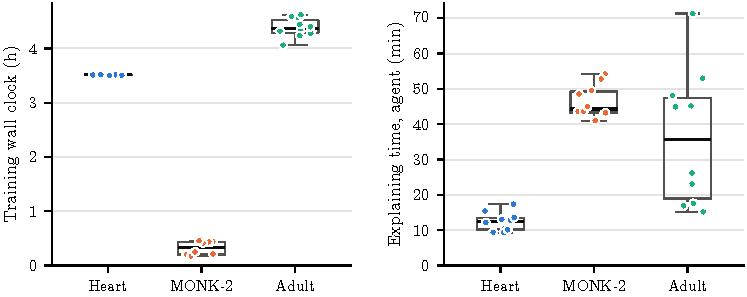
\includegraphics[width=\textwidth,height=0.8\textheight,keepaspectratio]{figures/ch7/10seed-cost_prereg.pdf}
  \caption{Earlier ten-seed export: training and explaining time, pre-registered datasets. One dot per seed (ten per dataset, horizontal jitter only); box: interquartile range; thick line: median; whiskers: minimum to maximum.}
  \label{fig:ch7-10seed-cost_prereg}
\end{figure}

% Generated by thesis/ch7/exp1/make_figures.py -- do not edit by hand.
\begin{figure}[tbp]
  \centering
  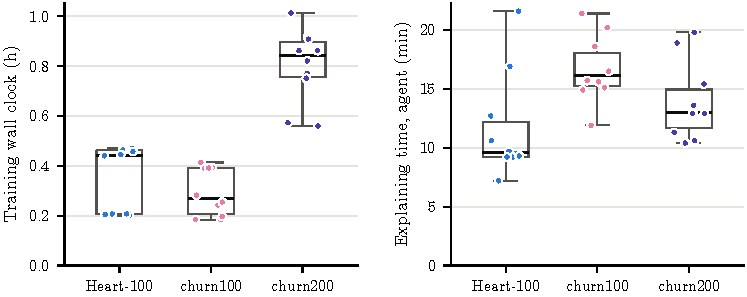
\includegraphics[width=\textwidth,height=0.8\textheight,keepaspectratio]{figures/ch7/options/10seed-cost_supp}
  \caption{Earlier ten-seed export: training and explaining time, additional analyses. One dot per seed (ten per dataset, horizontal jitter only); box: interquartile range; thick line: median; whiskers: minimum to maximum.}
  \label{fig:ch7-10seed-cost_supp}
\end{figure}

\clearpage
% Generated by thesis/ch7/exp1/make_figures.py -- do not edit by hand.
\begin{figure}[tbp]
  \centering
  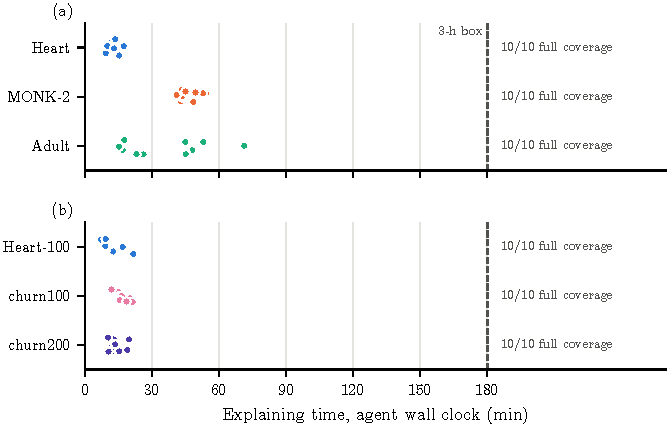
\includegraphics[width=\textwidth,height=0.8\textheight,keepaspectratio]{figures/ch7/options/10seed-coverage_time}
  \caption{Earlier ten-seed export: coverage against explaining time. One dot per network; filled: full coverage, hollow: not explained within the box. Dashed vertical line: the pre-registered time box. (a) Pre-registered datasets; (b) additional analyses.}
  \label{fig:ch7-10seed-coverage_time}
\end{figure}

% Generated by thesis/ch7/exp1/make_figures.py -- do not edit by hand.
\begin{figure}[tbp]
  \centering
  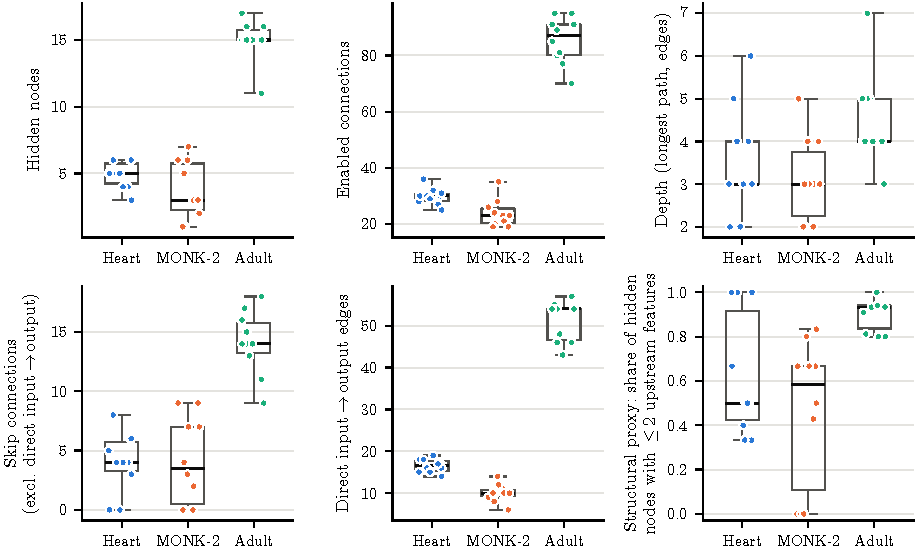
\includegraphics[width=\textwidth,height=0.8\textheight,keepaspectratio]{figures/ch7/options/10seed-structure_prereg}
  \caption{Earlier ten-seed export: network structure, pre-registered datasets. One dot per seed (ten per dataset, horizontal jitter only); box: interquartile range; thick line: median; whiskers: minimum to maximum. Open diamond: the paper's network for that dataset.}
  \label{fig:ch7-10seed-structure_prereg}
\end{figure}

\clearpage
% Generated by thesis/ch7/exp1/make_figures.py -- do not edit by hand.
\begin{figure}[tbp]
  \centering
  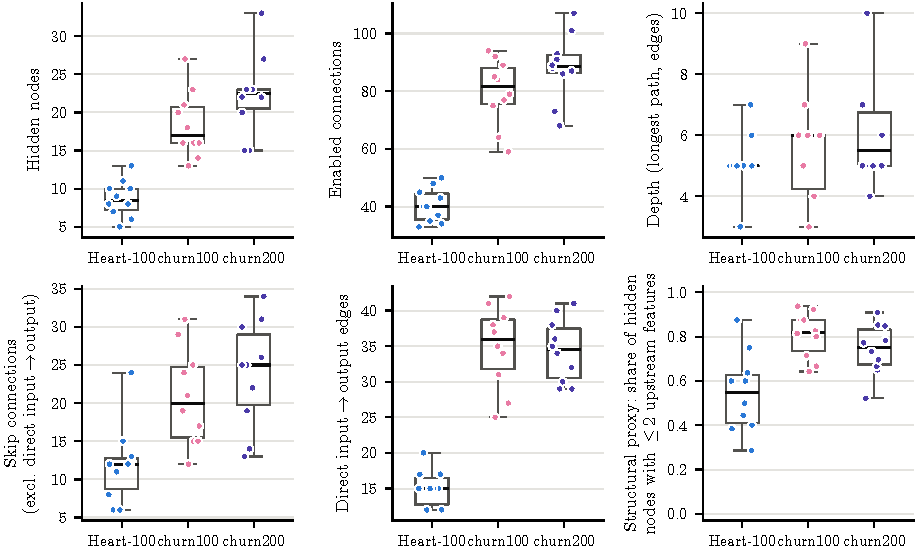
\includegraphics[width=\textwidth,height=0.8\textheight,keepaspectratio]{figures/ch7/10seed-structure_supp.pdf}
  \caption{Earlier ten-seed export: network structure, additional analyses. One dot per seed (ten per dataset, horizontal jitter only); box: interquartile range; thick line: median; whiskers: minimum to maximum.}
  \label{fig:ch7-10seed-structure_supp}
\end{figure}

% Generated by thesis/ch7/exp1/make_figures.py -- do not edit by hand.
\begin{figure}[tbp]
  \centering
  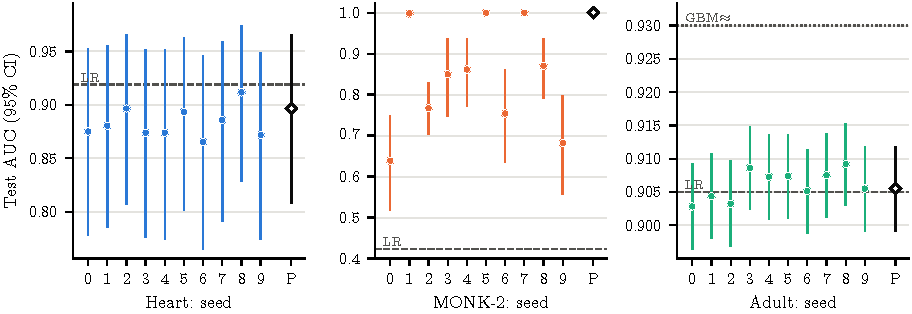
\includegraphics[width=\textwidth,height=0.8\textheight,keepaspectratio]{figures/ch7/options/10seed-test_auc_prereg}
  \caption{Earlier ten-seed export: test AUC per seed, pre-registered datasets. Dots and bars: each seed's test AUC with its 95\% interval. Dashed: L2 logistic regression (LR); dotted: gradient boosting (GBM; $\approx$: approximate, not the same split).}
  \label{fig:ch7-10seed-test_auc_prereg}
\end{figure}

\clearpage
% Generated by thesis/ch7/exp1/make_figures.py -- do not edit by hand.
\begin{figure}[tbp]
  \centering
  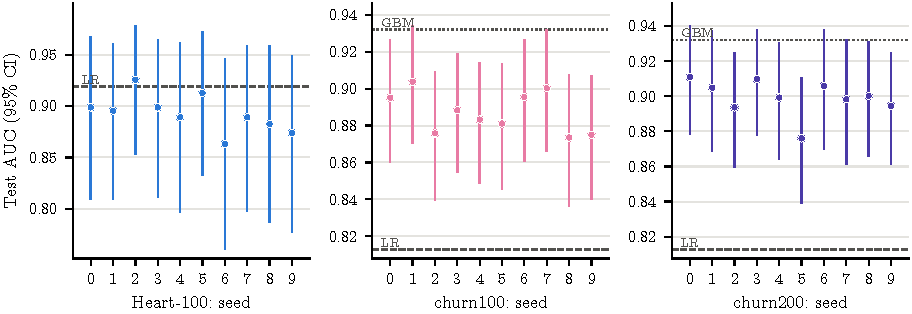
\includegraphics[width=\textwidth,height=0.8\textheight,keepaspectratio]{figures/ch7/10seed-test_auc_supp.pdf}
  \caption{Earlier ten-seed export: test AUC per seed, additional analyses. Dots and bars: each seed's test AUC with its 95\% interval. Dashed: L2 logistic regression (LR); dotted: gradient boosting (GBM).}
  \label{fig:ch7-10seed-test_auc_supp}
\end{figure}

% Generated by thesis/ch7/exp1/bench_figures.py -- do not edit by hand.
\begin{figure}[tbp]
  \centering
  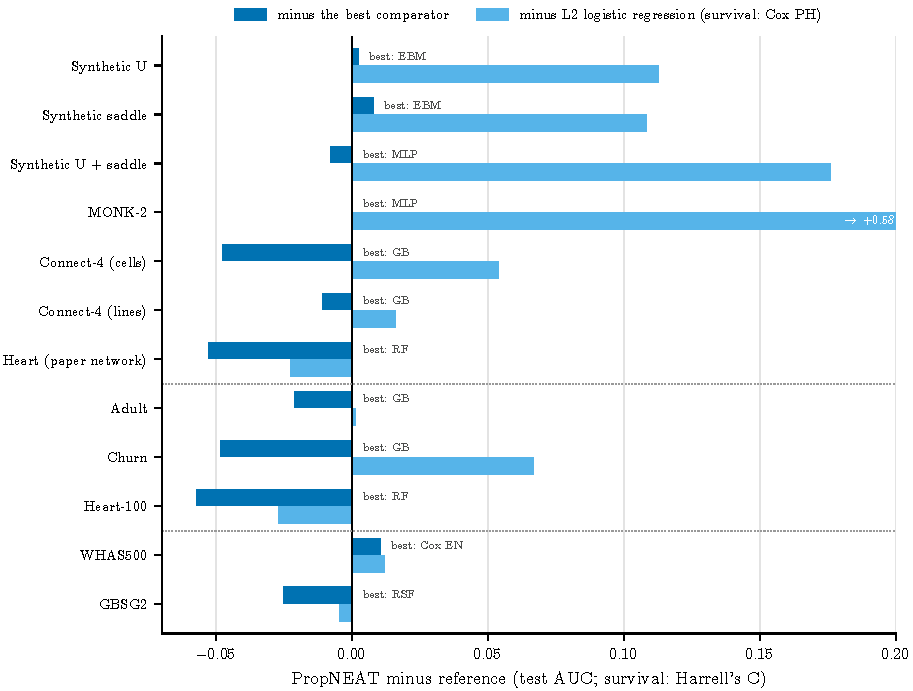
\includegraphics[width=\textwidth,height=0.8\textheight,keepaspectratio]{figures/ch7/options/bench-gap}
  \caption{PropNEAT's test AUC minus the best comparator's and logistic regression's. Dark blue: minus the best comparator (named); light blue: minus logistic regression (survival: Cox PH, Harrell's C); arrow: a bar cut at 0.2, its value printed. LR: logistic regression ($L_2$); L1: $L_1$ logistic regression; RF: random forest; GB: gradient boosting; EBM: explainable boosting machine; MLP: multilayer perceptron; Cox L2 / Cox EN: Cox model with a ridge / elastic-net penalty; RSF: random survival forest; GBS: gradient-boosted survival model.}
  \label{fig:ch7-bench-gap}
\end{figure}

\clearpage
% Generated by thesis/ch7/exp2/exp2_figures.py -- do not edit by hand.
\begin{figure}[tbp]
  \centering
  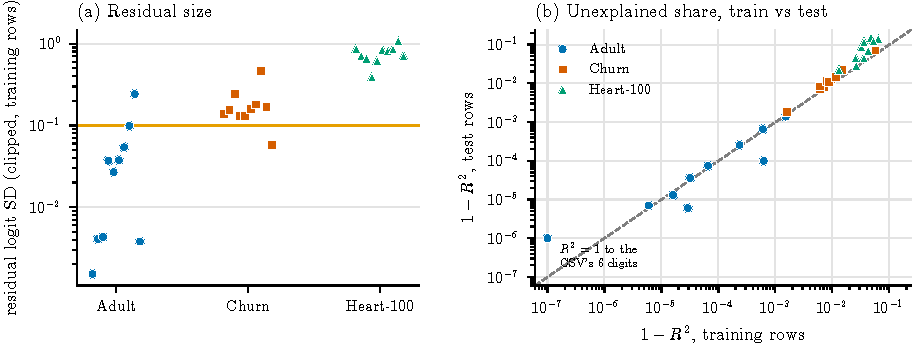
\includegraphics[width=\textwidth,height=0.8\textheight,keepaspectratio]{figures/ch7/options/completeness-residual}
  \caption{Residual of the signal catalogue, per network. (a) Residual logit SD (log scale); orange line: 0.10. (b) $1 - R^2$ on training against test rows (log scales); dashed: equal. Colour and marker: dataset.}
  \label{fig:ch7-completeness-residual}
\end{figure}

% Generated by thesis/ch7/exp2/exp2_figures.py -- do not edit by hand.
\begin{figure}[tbp]
  \centering
  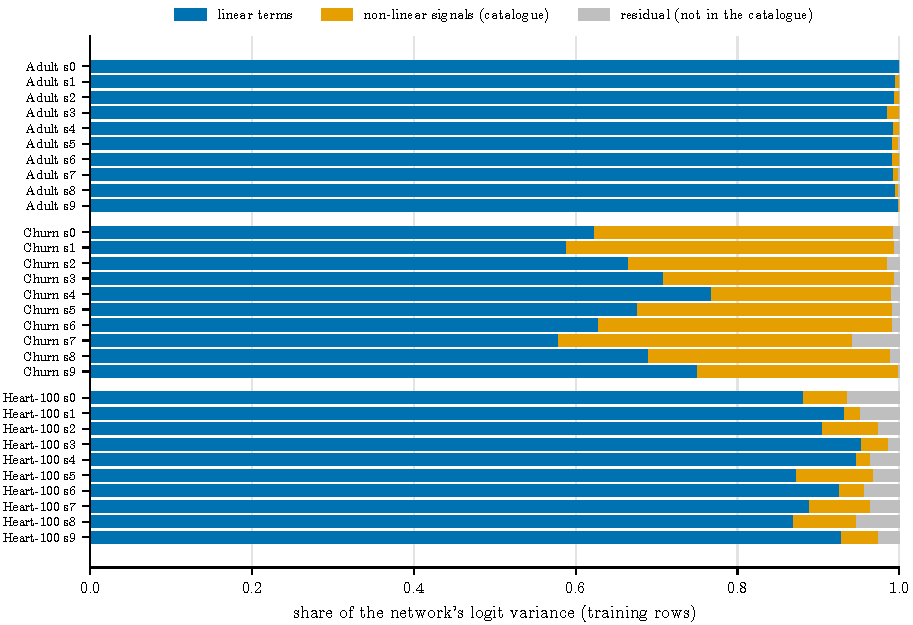
\includegraphics[width=\textwidth,height=0.8\textheight,keepaspectratio]{figures/ch7/completeness-shares.pdf}
  \caption{Shares of each network's logit variance (training rows). Blue: linear terms; orange: non-linear signals of the catalogue; grey: residual.}
  \label{fig:ch7-completeness-shares}
\end{figure}

\clearpage
% Generated by thesis/ch7/exp1/bench_figures.py -- do not edit by hand.
\begin{figure}[tbp]
  \centering
  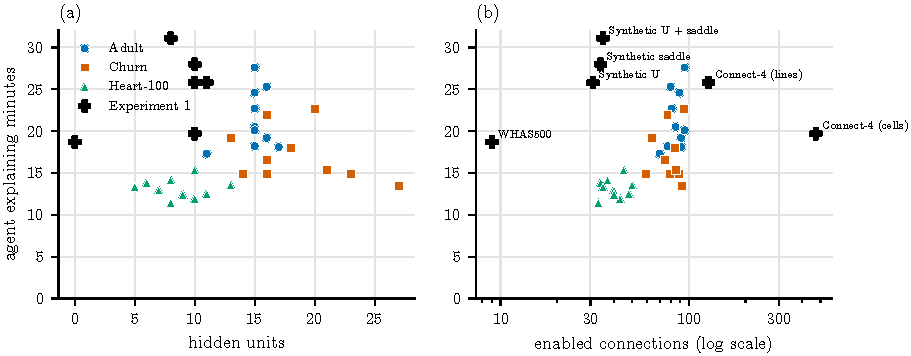
\includegraphics[width=\textwidth,height=0.8\textheight,keepaspectratio]{figures/ch7/options/cost-minutes-size}
  \caption{Explaining minutes against network size, Experiments 1 and 2. Colour and marker: Experiment 2 dataset; black plus: an Experiment 1 network (named in b); (b) log scale.}
  \label{fig:ch7-cost-minutes-size}
\end{figure}

% Generated by thesis/ch7/exp2/exp2_figures.py -- do not edit by hand.
\begin{figure}[tbp]
  \centering
  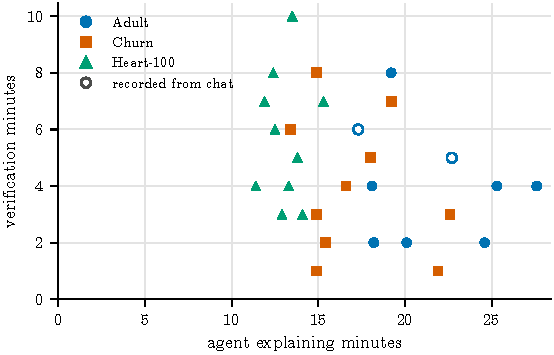
\includegraphics[width=\textwidth,height=0.8\textheight,keepaspectratio]{figures/ch7/options/cost-verify}
  \caption{Verification minutes against explaining minutes. Colour and marker: dataset; open: minutes recorded from chat.}
  \label{fig:ch7-cost-verify}
\end{figure}

\clearpage
% Generated by thesis/ch7/exp1/make_figures.py -- do not edit by hand.
\begin{figure}[tbp]
  \centering
  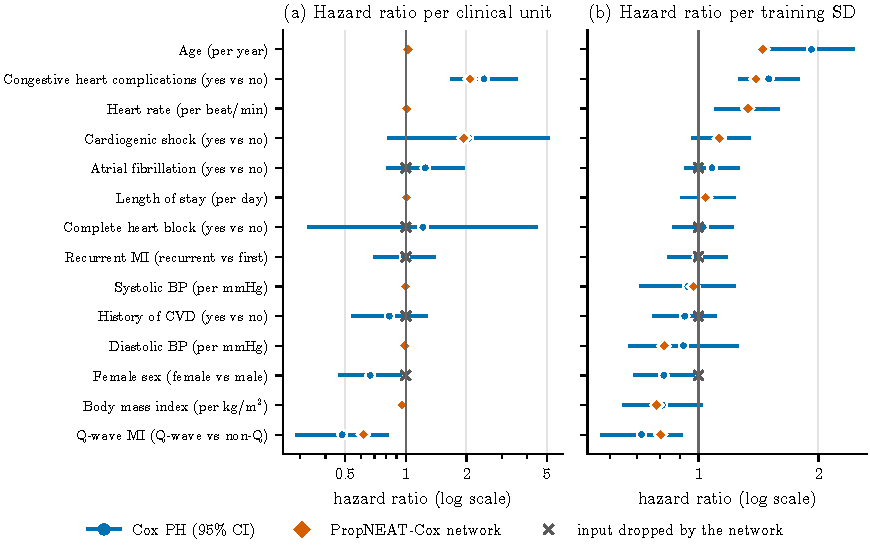
\includegraphics[width=\textwidth,height=0.8\textheight,keepaspectratio]{figures/ch7/options/cox-whas500-forest}
  \caption{WHAS500: hazard ratios of Cox PH and of the PropNEAT-Cox network, training rows ($n$ = 320). Blue dot and bar: the Cox PH hazard ratio with its 95\% interval; red diamond: the network's hazard ratio; cross at 1: an input the network does not use. Log scale; vertical line: 1.}
  \label{fig:ch7-cox-whas500-forest}
\end{figure}

% Generated by thesis/ch7/exp1/make_figures.py -- do not edit by hand.
\begin{figure}[tbp]
  \centering
  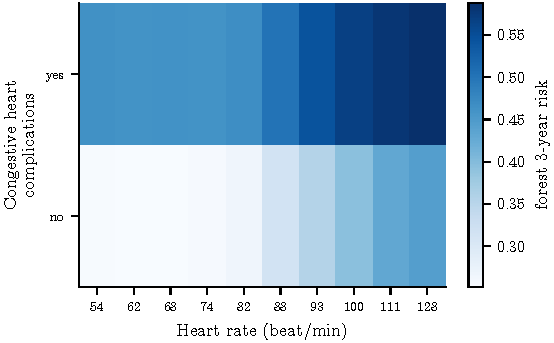
\includegraphics[width=0.6\textwidth,height=0.8\textheight,keepaspectratio]{figures/ch7/cox-whas500-h2d.pdf}
  \caption{WHAS500: the forest's strongest pair, two-way partial dependence. Colour: the random survival forest's predicted 3-year risk, averaged over the training patients with the two inputs set to each cell's values (darker: higher).}
  \label{fig:ch7-cox-whas500-h2d}
\end{figure}

\clearpage
% Generated by thesis/ch7/exp1/make_figures.py -- do not edit by hand.
\begin{figure}[tbp]
  \centering
  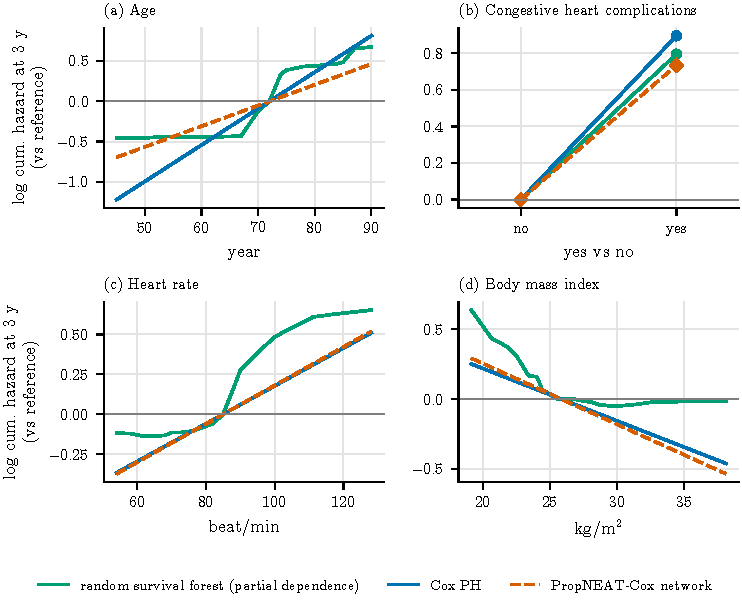
\includegraphics[width=\textwidth,height=0.8\textheight,keepaspectratio]{figures/ch7/options/cox-whas500-pd}
  \caption{WHAS500: the forest's top inputs, partial dependence at 3 years. Green: the random survival forest's partial dependence; blue: Cox PH; red dashed: the network. Each curve is relative to the reference value (the lower level; the training median).}
  \label{fig:ch7-cox-whas500-pd}
\end{figure}

% Generated by thesis/ch7/exp1/make_figures.py -- do not edit by hand.
\begin{figure}[tbp]
  \centering
  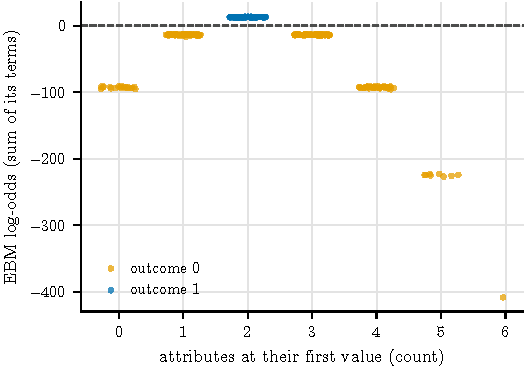
\includegraphics[width=0.65\textwidth,height=0.8\textheight,keepaspectratio]{figures/ch7/ebm-monk2-count.pdf}
  \caption{MONK-2: the explainable boosting machine on the six raw attributes (6 main terms, 15 pairwise terms), its log-odds against the count of attributes at their first value. One point per training row, jittered horizontally; blue: outcome 1; orange: outcome 0; dashed: log-odds 0.}
  \label{fig:ch7-ebm-monk2-count}
\end{figure}

\clearpage
% Generated by thesis/ch7/exp1/make_figures.py -- do not edit by hand.
\begin{figure}[tbp]
  \centering
  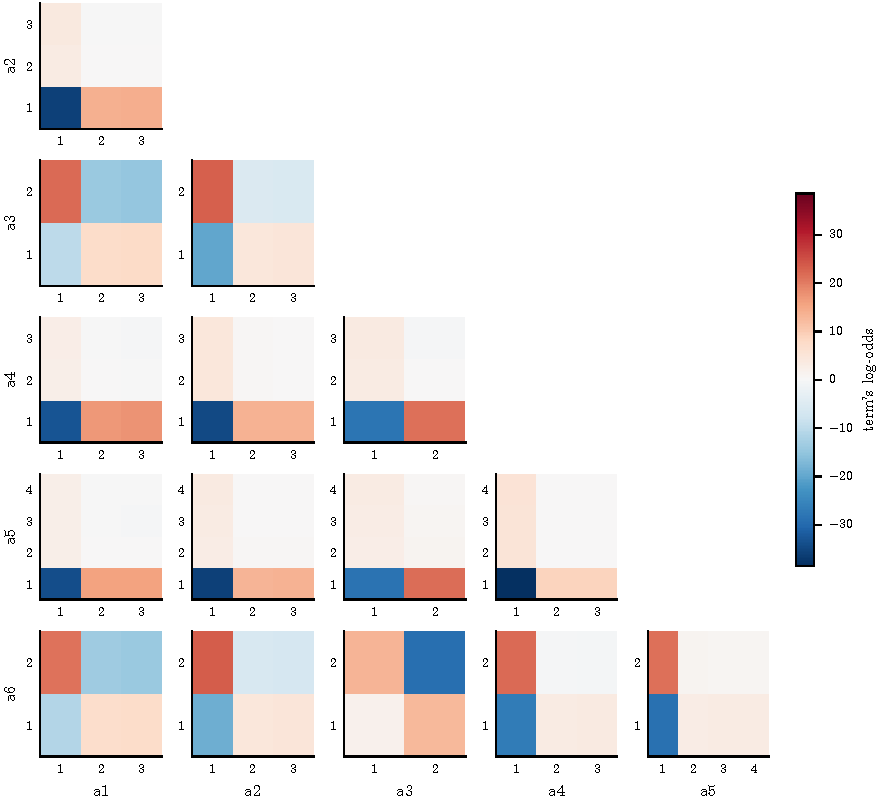
\includegraphics[width=\textwidth,height=0.8\textheight,keepaspectratio]{figures/ch7/ebm-monk2-pairs.pdf}
  \caption{MONK-2: the 15 pairwise terms of the explainable boosting machine on the six raw attributes. One panel per pair of attributes $a_i$ (across) and $a_j$ (up), each axis the attribute's values, value 1 (the first value) at the lower left; colour: the term's log-odds (red raises, blue lowers), one scale for all panels.}
  \label{fig:ch7-ebm-monk2-pairs}
\end{figure}

% Generated by thesis/ch7/exp2/make_assets.py -- do not edit by hand.
\begin{figure}[tbp]
  \centering
  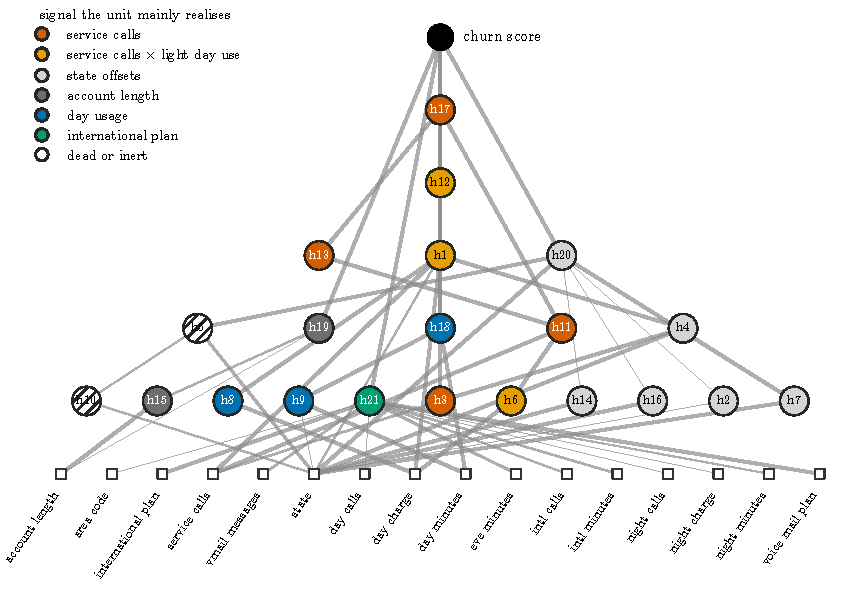
\includegraphics[width=\textwidth,height=0.8\textheight,keepaspectratio]{figures/ch7/exp2-churn-s5-network.pdf}
  \caption{Churn seed 5: every hidden node, coloured by the signal it mainly realises. The 31 state indicators are drawn as one input; line width: absolute weight.}
  \label{fig:exp2-churn-s5-network}
\end{figure}

\clearpage
% Generated by thesis/ch7/exp2/make_assets.py -- do not edit by hand.
\begin{figure}[tbp]
  \centering
  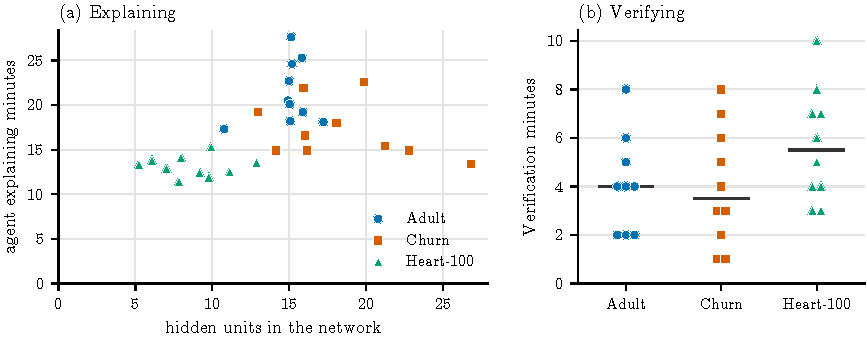
\includegraphics[width=\textwidth,height=0.8\textheight,keepaspectratio]{figures/ch7/options/exp2-cost}
  \caption{Cost of explaining and verifying, one mark per network. (a) The explaining agent's minutes against network size. (b) Verification minutes; bar: median per study.}
  \label{fig:exp2-cost}
\end{figure}

% Generated by thesis/ch7/exp2/make_assets.py -- do not edit by hand.
\begin{figure}[tbp]
  \centering
  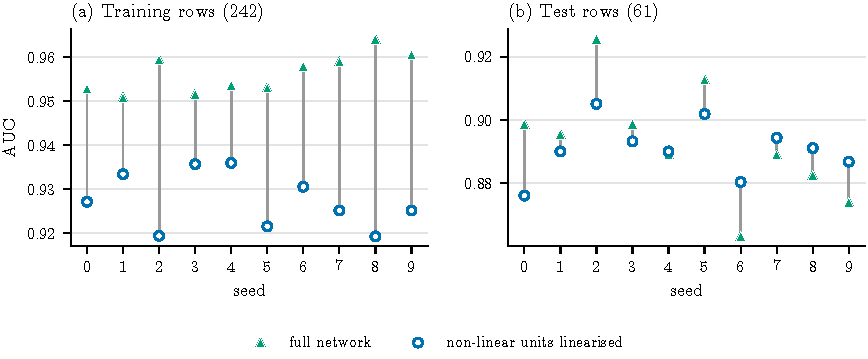
\includegraphics[width=\textwidth,height=0.8\textheight,keepaspectratio]{figures/ch7/exp2-heart-linearised.pdf}
  \caption{Heart-100: each network's AUC with and without its non-linear units.}
  \label{fig:exp2-heart-linearised}
\end{figure}

\clearpage
% Generated by thesis/ch7/exp2/make_assets.py -- do not edit by hand.
\begin{figure}[tbp]
  \centering
  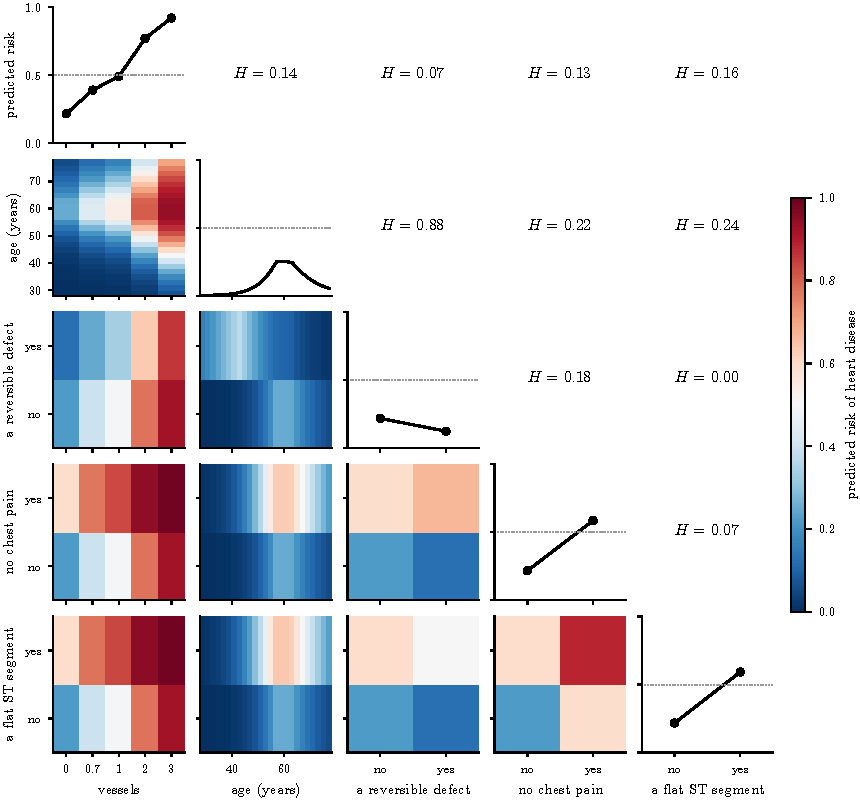
\includegraphics[width=0.95\textwidth,height=0.8\textheight,keepaspectratio]{figures/ch7/exp2-heart-pairs.pdf}
  \caption{Heart-100 seed 2, the whole model: a pairs plot over 5 inputs. Diagonal: predicted risk as one input varies; below the diagonal: as two vary together (colour, centred on a risk of 0.5); above the diagonal: the interaction strength $H$.}
  \label{fig:exp2-heart-pairs}
\end{figure}

% Generated by thesis/ch7/exp2/exp2_figures.py -- do not edit by hand.
\begin{figure}[tbp]
  \centering
  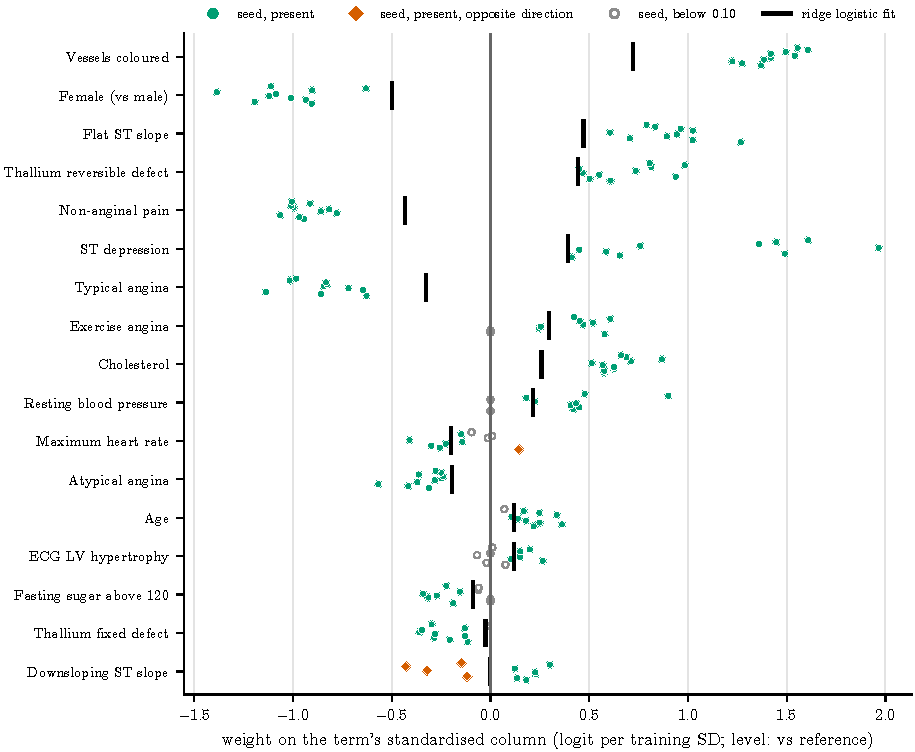
\includegraphics[width=\textwidth,height=0.8\textheight,keepaspectratio]{figures/ch7/heart-lincore-vs-data.pdf}
  \caption{Heart-100: weight of each linear term in each seed's network and in a ridge logistic fit. Green: a seed with the term present ($\geq$ 0.10); red diamond: present, opposite direction to most seeds; open: below 0.10; black bar: ridge logistic fit.}
  \label{fig:ch7-heart-lincore-vs-data}
\end{figure}

\clearpage
% Generated by thesis/ch7/exp1/bench_figures.py -- do not edit by hand.
\begin{figure}[tbp]
  \centering
  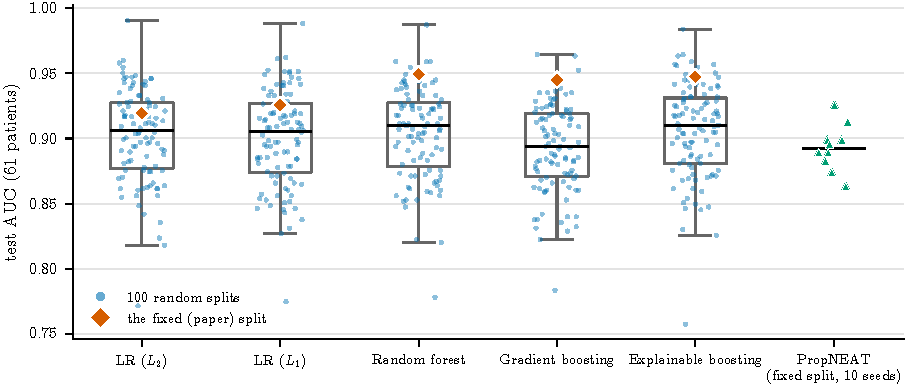
\includegraphics[width=\textwidth,height=0.8\textheight,keepaspectratio]{figures/ch7/options/heart-splits-box}
  \caption{Heart: test AUC of each comparator over random splits. Box and blue points: 100 random splits (61 test patients); red diamond: the fixed split; green triangles: the ten Heart-100 seeds on the fixed split, bar: their median.}
  \label{fig:ch7-heart-splits-box}
\end{figure}

% Generated by thesis/ch7/exp1/bench_figures.py -- do not edit by hand.
\begin{figure}[tbp]
  \centering
  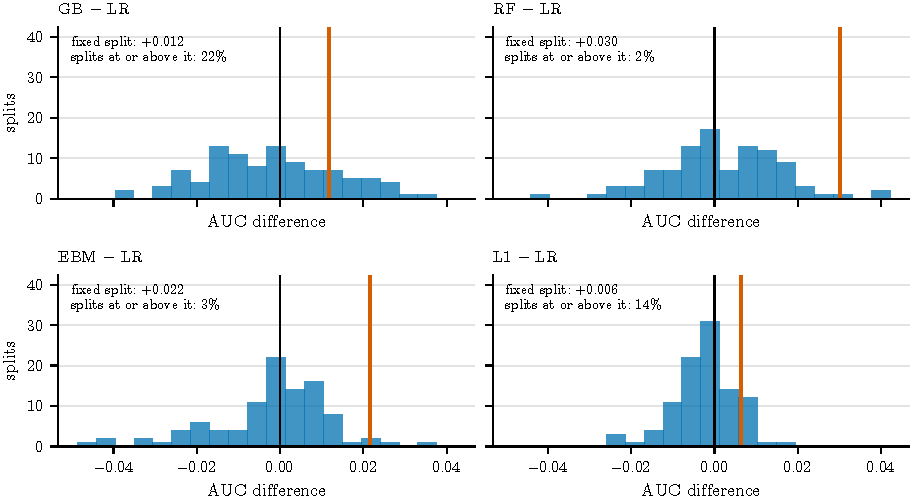
\includegraphics[width=\textwidth,height=0.8\textheight,keepaspectratio]{figures/ch7/heart-splits-diff.pdf}
  \caption{Heart: test AUC minus logistic regression's over random splits. Histogram: 100 random splits; red line: the fixed split; black line: zero.}
  \label{fig:ch7-heart-splits-diff}
\end{figure}

\clearpage
% Generated by thesis/ch7/exp2/exp2_figures.py -- do not edit by hand.
\begin{figure}[tbp]
  \centering
  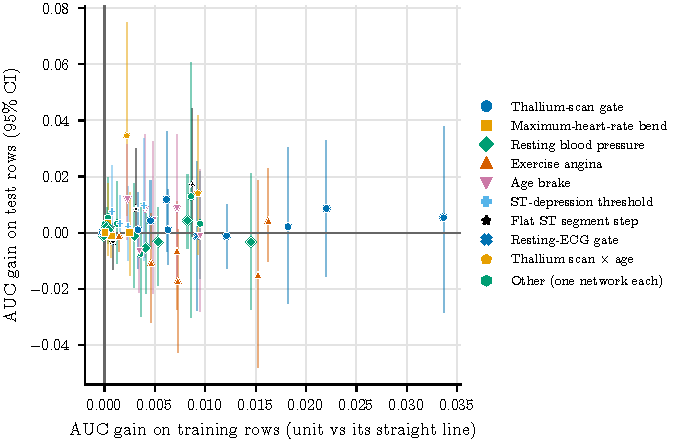
\includegraphics[width=\textwidth,height=0.8\textheight,keepaspectratio]{figures/ch7/heart-units-gain.pdf}
  \caption{Heart-100: AUC gain of each non-linear unit over its straight line, training against test rows. Colour and marker: family; vertical line: 95\% interval of the test gain.}
  \label{fig:ch7-heart-units-gain}
\end{figure}

% Generated by thesis/ch7/exp2/exp2_figures.py -- do not edit by hand.
\begin{figure}[tbp]
  \centering
  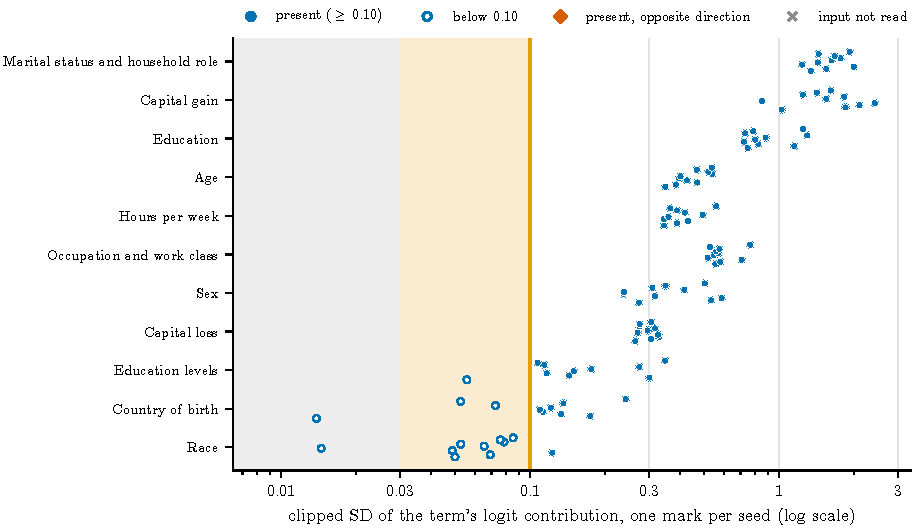
\includegraphics[width=\textwidth,height=0.8\textheight,keepaspectratio]{figures/ch7/lincore-adult.pdf}
  \caption{Adult: size of each linear term in each seed's network. One mark per seed (log scale). Filled blue: present ($\geq$ 0.10); open: below 0.10; red diamond: present, opposite direction to most seeds; $\times$: input not read. Shading: below 0.03 (grey) and 0.03--0.10 (orange); orange line: 0.10.}
  \label{fig:ch7-lincore-adult}
\end{figure}

\clearpage
% Generated by thesis/ch7/exp2/exp2_figures.py -- do not edit by hand.
\begin{figure}[tbp]
  \centering
  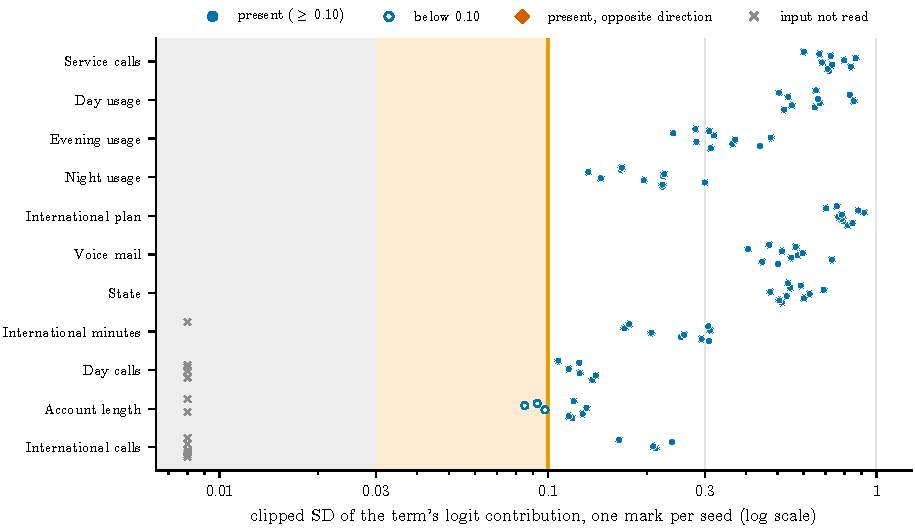
\includegraphics[width=\textwidth,height=0.8\textheight,keepaspectratio]{figures/ch7/options/lincore-churn}
  \caption{Churn: size of each linear term in each seed's network. One mark per seed (log scale). Filled blue: present ($\geq$ 0.10); open: below 0.10; red diamond: present, opposite direction to most seeds; $\times$: input not read. Shading: below 0.03 (grey) and 0.03--0.10 (orange); orange line: 0.10.}
  \label{fig:ch7-lincore-churn}
\end{figure}

% Generated by thesis/ch7/exp2/exp2_figures.py -- do not edit by hand.
\begin{figure}[tbp]
  \centering
  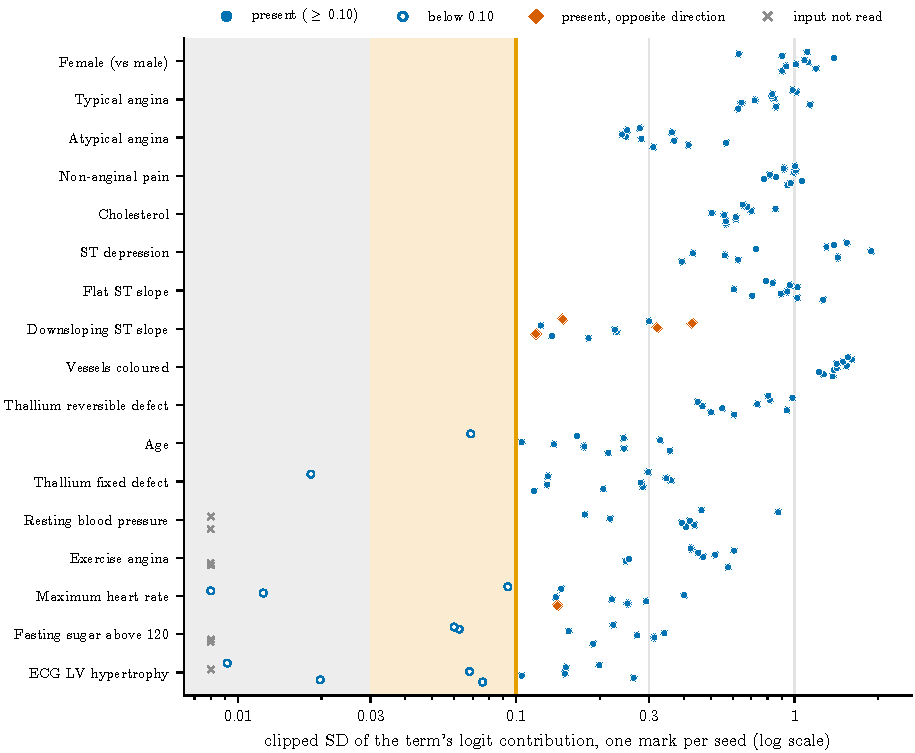
\includegraphics[width=\textwidth,height=0.8\textheight,keepaspectratio]{figures/ch7/lincore-heart100.pdf}
  \caption{Heart-100: size of each linear term in each seed's network. One mark per seed (log scale). Filled blue: present ($\geq$ 0.10); open: below 0.10; red diamond: present, opposite direction to most seeds; $\times$: input not read. Shading: below 0.03 (grey) and 0.03--0.10 (orange); orange line: 0.10.}
  \label{fig:ch7-lincore-heart100}
\end{figure}

\clearpage
% Generated by thesis/ch7/exp2/exp2_figures.py -- do not edit by hand.
\begin{figure}[tbp]
  \centering
  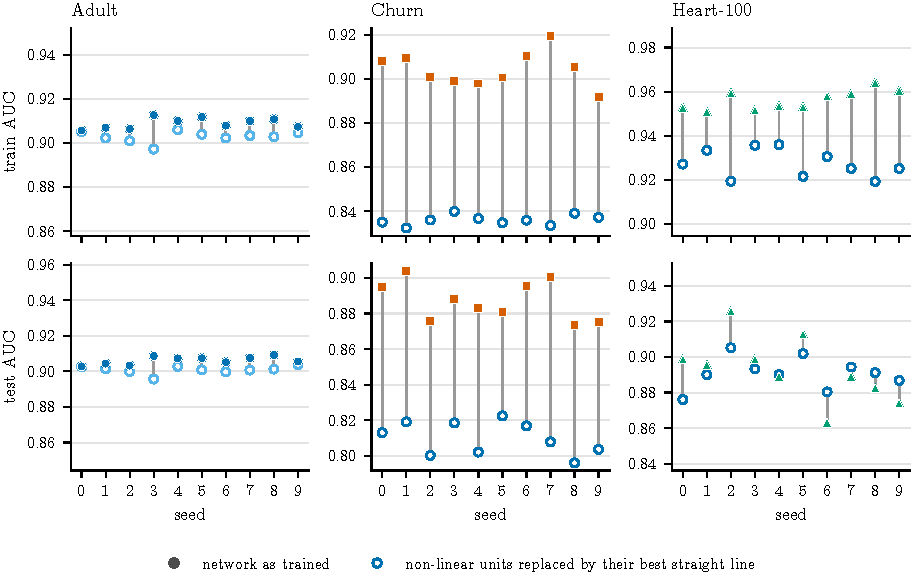
\includegraphics[width=\textwidth,height=0.8\textheight,keepaspectratio]{figures/ch7/options/linearised-auc}
  \caption{AUC of each network as trained and with its non-linear units linearised. Filled: the network as trained; open: every non-linear unit replaced by its best straight line; grey: joins a seed's two values. The panels of a row span the same AUC range.}
  \label{fig:ch7-linearised-auc}
\end{figure}

% Generated by thesis/ch7/exp2/exp2_figures.py -- do not edit by hand.
\begin{figure}[tbp]
  \centering
  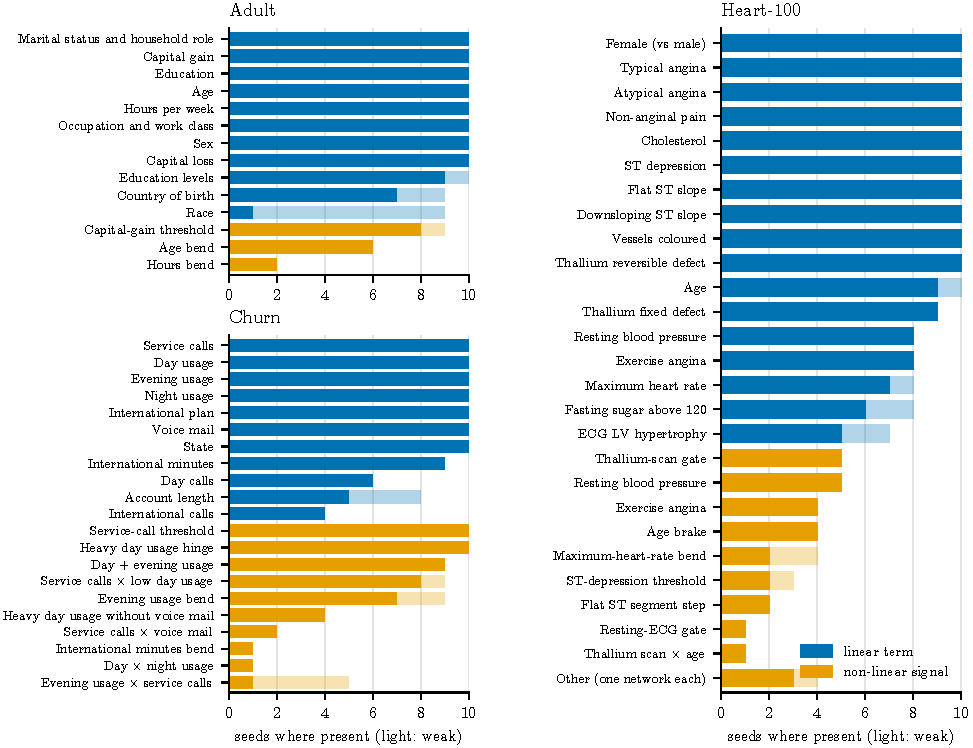
\includegraphics[width=\textwidth,height=0.8\textheight,keepaspectratio]{figures/ch7/recurrence.pdf}
  \caption{Number of seeds carrying each signal. Bar: seeds where the signal is present; light extension: seeds where it is weak. Blue: linear term; orange: non-linear signal.}
  \label{fig:ch7-recurrence}
\end{figure}

\clearpage
% Generated by thesis/ch7/exp2/exp2_figures.py -- do not edit by hand.
\begin{figure}[tbp]
  \centering
  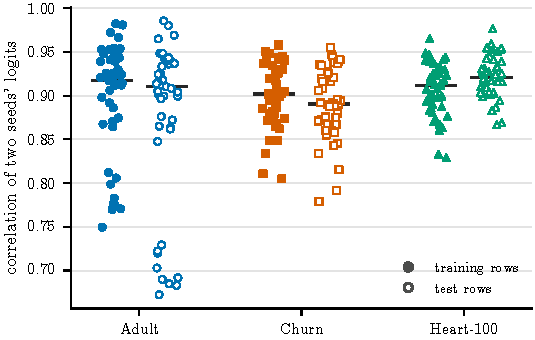
\includegraphics[width=\textwidth,height=0.8\textheight,keepaspectratio]{figures/ch7/seed-agreement-strip.pdf}
  \caption{Pairwise correlation of the ten networks' logits, training and test rows. One mark per pair of seeds; filled: training rows; open: test rows; bar: median.}
  \label{fig:ch7-seed-agreement-strip}
\end{figure}

% Generated by thesis/ch7/exp2/exp2_figures.py -- do not edit by hand.
\begin{figure}[tbp]
  \centering
  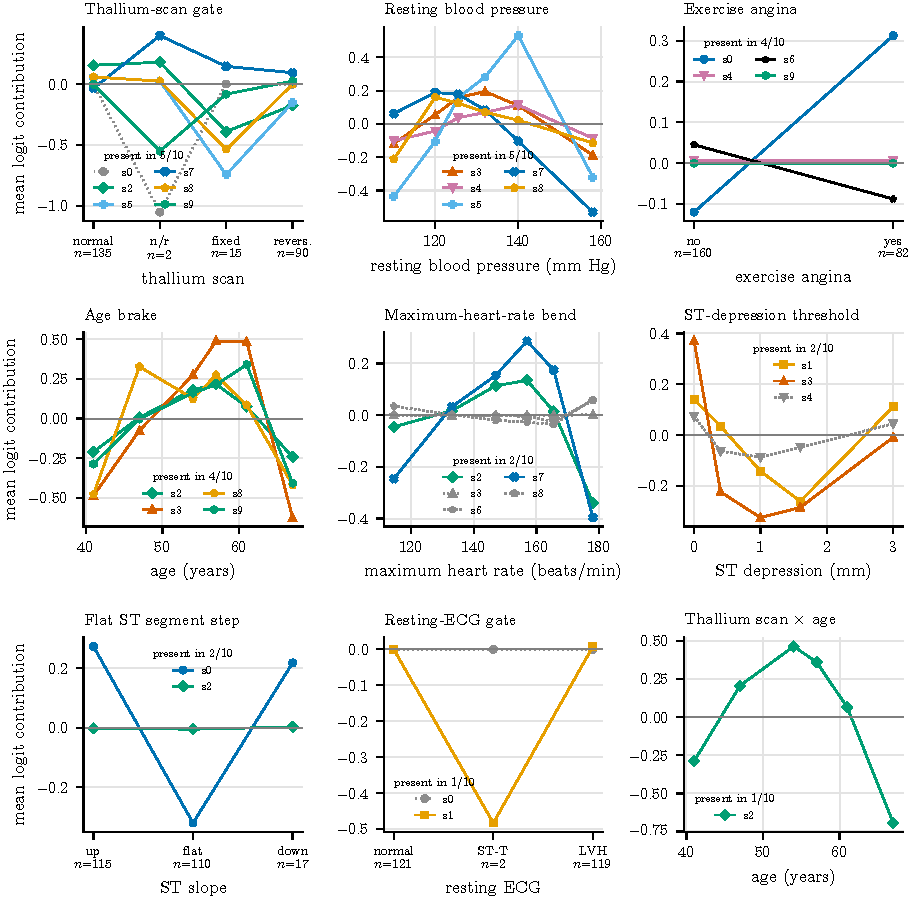
\includegraphics[width=\textwidth,height=0.8\textheight,keepaspectratio]{figures/ch7/options/sig-shapes-heart100}
  \caption{Heart-100: shapes of the non-linear families, one line per seed. Mean logit contribution of the family in each quantile band (numeric input, drawn at the band's median) or level of its main input; colour and marker: seed; grey dotted: weak.}
  \label{fig:ch7-sig-shapes-heart100}
\end{figure}

\clearpage
% Generated by thesis/ch7/exp2/exp2_figures.py -- do not edit by hand.
\begin{figure}[tbp]
  \centering
  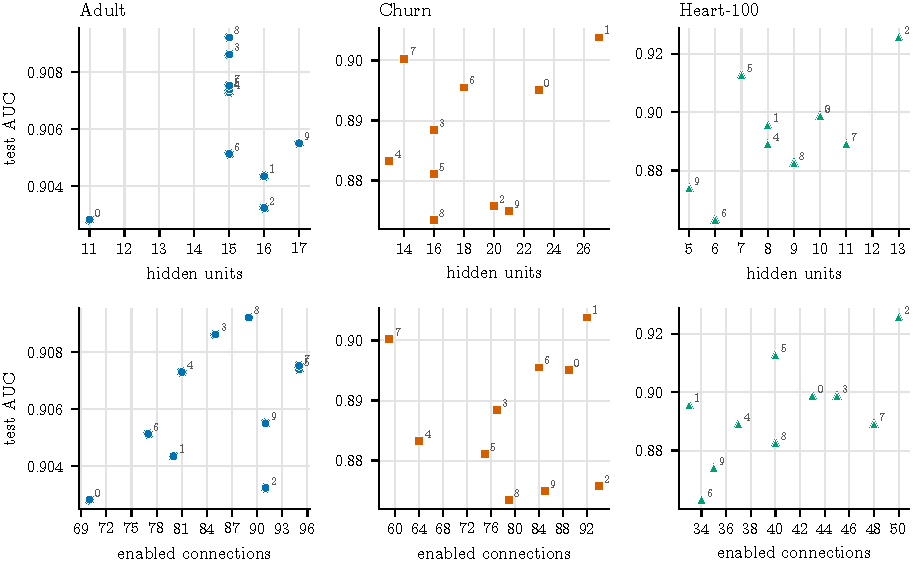
\includegraphics[width=\textwidth,height=0.8\textheight,keepaspectratio]{figures/ch7/size-vs-auc.pdf}
  \caption{Network size against test AUC. Numbers beside the marks: seed.}
  \label{fig:ch7-size-vs-auc}
\end{figure}

% Generated by thesis/ch7/exp1/make_figures.py -- do not edit by hand.
\begin{figure}[tbp]
  \centering
  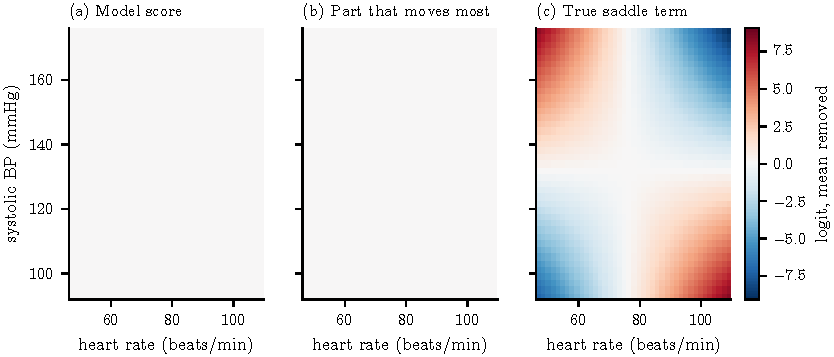
\includegraphics[width=\textwidth,height=0.8\textheight,keepaspectratio]{figures/ch7/options/synthetic-shape-a-saddle}
  \caption{Synthetic data (U only), the explained network: heart rate $\times$ systolic BP. Colour: the logit with its mean over the grid removed, one scale for all panels (red above the mean, blue below); every other input at the typical case. (b) The explanation part whose contribution moves most on the grid (\emph{sodium U}). This dataset has no saddle term; (c) shows it for comparison. True term: $-1.5\,z_h z_p$ (standardised heart rate and systolic BP).}
  \label{fig:ch7-synthetic-shape-a-saddle}
\end{figure}

\clearpage
% Generated by thesis/ch7/exp1/make_figures.py -- do not edit by hand.
\begin{figure}[tbp]
  \centering
  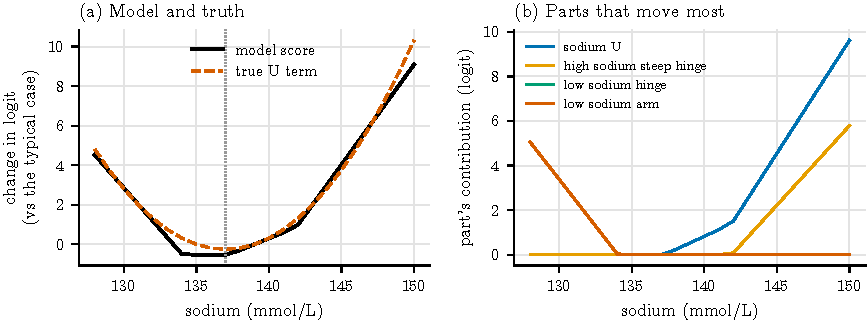
\includegraphics[width=\textwidth,height=0.8\textheight,keepaspectratio]{figures/ch7/synthetic-shape-a-sodium.pdf}
  \caption{Synthetic data (U only), the explained network: response to sodium. Black: the model's score as sodium varies, every other input at the typical case, relative to the typical sodium; dashed: the true U term $((z_n - (-0.5))^2 - 1)$, lowest at 137 mmol/L; dotted: 137 mmol/L. (b) The explanation parts whose contribution moves most with sodium.}
  \label{fig:ch7-synthetic-shape-a-sodium}
\end{figure}

% Generated by thesis/ch7/exp1/make_figures.py -- do not edit by hand.
\begin{figure}[tbp]
  \centering
  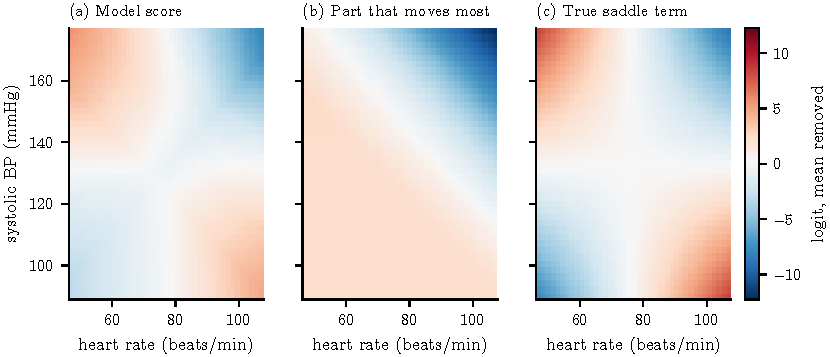
\includegraphics[width=\textwidth,height=0.8\textheight,keepaspectratio]{figures/ch7/options/synthetic-shape-b-saddle}
  \caption{Synthetic data (saddle only), the explained network: heart rate $\times$ systolic BP. Colour: the logit with its mean over the grid removed, one scale for all panels (red above the mean, blue below); every other input at the typical case. (b) The explanation part whose contribution moves most on the grid (\emph{pressure rate load}). True term: $-1.5\,z_h z_p$ (standardised heart rate and systolic BP).}
  \label{fig:ch7-synthetic-shape-b-saddle}
\end{figure}

\clearpage
% Generated by thesis/ch7/exp1/make_figures.py -- do not edit by hand.
\begin{figure}[tbp]
  \centering
  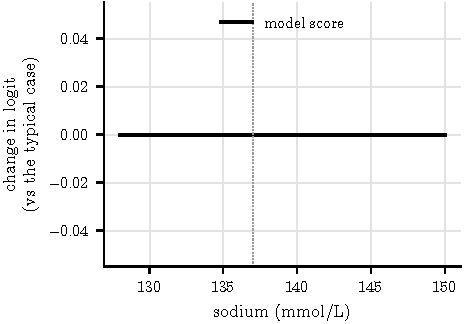
\includegraphics[width=\textwidth,height=0.8\textheight,keepaspectratio]{figures/ch7/options/synthetic-shape-b-sodium}
  \caption{Synthetic data (saddle only), the explained network: response to sodium. Black: the model's score as sodium varies, every other input at the typical case, relative to the typical sodium; dotted: 137 mmol/L. This dataset has no U term.}
  \label{fig:ch7-synthetic-shape-b-sodium}
\end{figure}

% Generated by thesis/ch7/exp1/make_figures.py -- do not edit by hand.
\begin{figure}[tbp]
  \centering
  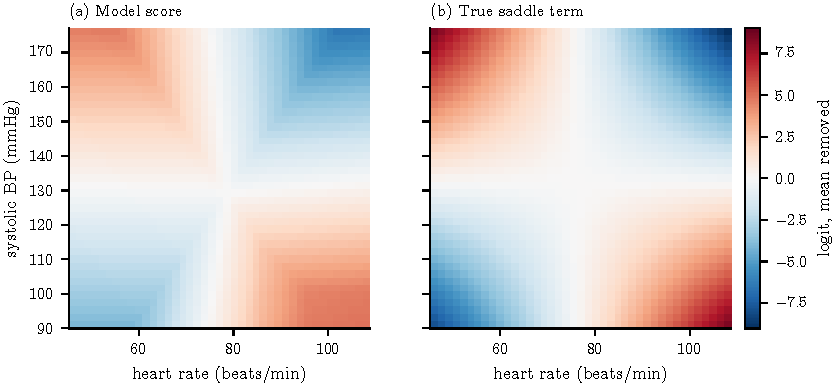
\includegraphics[width=\textwidth,height=0.8\textheight,keepaspectratio]{figures/ch7/options/synthetic-shape-c-s1-g300-saddle}
  \caption{Synthetic data (U and saddle), seed 1 at generation 300 (not explained): heart rate $\times$ systolic BP. Colour: the logit with its mean over the grid removed, one scale for all panels (red above the mean, blue below); every other input at the typical case. True term: $-1.5\,z_h z_p$ (standardised heart rate and systolic BP).}
  \label{fig:ch7-synthetic-shape-c-s1-g300-saddle}
\end{figure}

\clearpage
% Generated by thesis/ch7/exp1/make_figures.py -- do not edit by hand.
\begin{figure}[tbp]
  \centering
  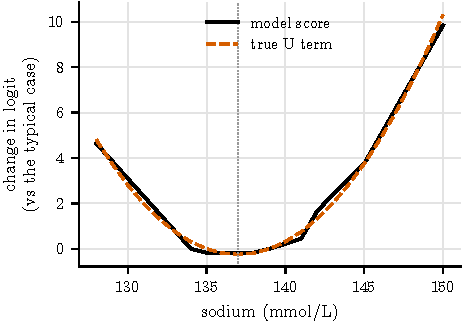
\includegraphics[width=\textwidth,height=0.8\textheight,keepaspectratio]{figures/ch7/options/synthetic-shape-c-s1-g300-sodium}
  \caption{Synthetic data (U and saddle), seed 1 at generation 300 (not explained): response to sodium. Black: the model's score as sodium varies, every other input at the typical case, relative to the typical sodium; dashed: the true U term $((z_n - (-0.5))^2 - 1)$, lowest at 137 mmol/L; dotted: 137 mmol/L.}
  \label{fig:ch7-synthetic-shape-c-s1-g300-sodium}
\end{figure}

% Generated by thesis/ch7/exp1/make_figures.py -- do not edit by hand.
\begin{figure}[tbp]
  \centering
  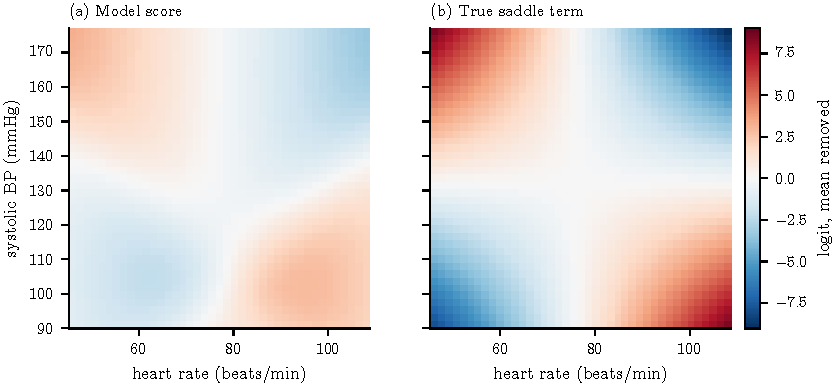
\includegraphics[width=\textwidth,height=0.8\textheight,keepaspectratio]{figures/ch7/options/synthetic-shape-c-sig-best-g300-saddle}
  \caption{Synthetic data (U and saddle), the best sigmoid-unit seed at generation 300 (not explained): heart rate $\times$ systolic BP. Colour: the logit with its mean over the grid removed, one scale for all panels (red above the mean, blue below); every other input at the typical case. True term: $-1.5\,z_h z_p$ (standardised heart rate and systolic BP).}
  \label{fig:ch7-synthetic-shape-c-sig-best-g300-saddle}
\end{figure}

\clearpage
% Generated by thesis/ch7/exp1/make_figures.py -- do not edit by hand.
\begin{figure}[tbp]
  \centering
  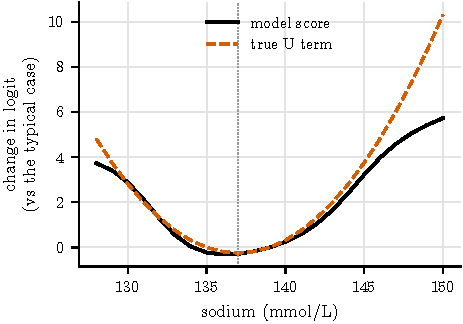
\includegraphics[width=\textwidth,height=0.8\textheight,keepaspectratio]{figures/ch7/options/synthetic-shape-c-sig-best-g300-sodium}
  \caption{Synthetic data (U and saddle), the best sigmoid-unit seed at generation 300 (not explained): response to sodium. Black: the model's score as sodium varies, every other input at the typical case, relative to the typical sodium; dashed: the true U term $((z_n - (-0.5))^2 - 1)$, lowest at 137 mmol/L; dotted: 137 mmol/L.}
  \label{fig:ch7-synthetic-shape-c-sig-best-g300-sodium}
\end{figure}

\clearpage
\end{document}
